%%%%%%%%%%%%%%%
% Parent document for the book Reproducible Research with R and RStudio
% Christopher Gandrud
% 14 January 2013
%%%%%%%%%%%%%%

% Tell RStudio that weaving is to be done with the knitr package
% !Rnw weave = knitr

% Load required LaTeX packages
\documentclass[krantz1]{krantz}
\usepackage[authoryear]{natbib}
\usepackage{amssymb}
\usepackage{amsmath}
\usepackage{graphicx}
%\usepackage{caption}
\usepackage{subfigure}
%\usepackage{epsfig}
\usepackage{makeidx}
%\usepackage{showidx}
\usepackage{multicol}
	\frenchspacing
	\tolerance=5000
\usepackage[usenames,dvipsnames,svgnames]{xcolor}
\usepackage{dcolumn}
\usepackage{booktabs}
\usepackage{multirow}
\usepackage{lscape}
\usepackage[hyphens]{url}
\usepackage{todonotes}
\usepackage{tikz}
	\usetikzlibrary{trees}
	\usetikzlibrary{decorations.pathmorphing}
	\usetikzlibrary{shapes,arrows}
\usepackage{wrapfig}
\usepackage{alltt}

\newcommand{\blankpage}{
	\newpage
	\thispagestyle{empty}
	\mbox{}
	\newpage
}


% Set margins on highlighted code output boxes
\setlength\fboxsep{6.25mm}

% Set knitr global options
\begin{knitrout}
\definecolor{shadecolor}{rgb}{0.969, 0.969, 0.969}\color{fgcolor}\begin{kframe}


{\ttfamily\noindent\bfseries\textcolor{errorcolor}{\#\# Error: object 'opts\_chunk' not found}}

{\ttfamily\noindent\bfseries\textcolor{errorcolor}{\#\# Error: object 'opts\_chunk' not found}}\end{kframe}
\end{knitrout}


\makeatletter
\makeatother
\makeindex

\begin{document}

% Title page
\title{Reproducible Research with R and RStudio}

\author{Christopher Gandrud}

\maketitle

% Set roman numeral page counter
\pagenumbering{roman}

% Front matter
\frontmatter

\blankpage
\blankpage
\blankpage
\blankpage

% Preface




\chapter*{Preface}

\todo[inline]{The preface is incomplete.}

\noindent This book would not have been possible without the advice and support of a great many people.

The developer and blogging community has been incredibly important for making this book possible. Foremost among among these people is Yihui Xie. He is the developer of the {\emph{knitr}} package (among others) and also an avid writer and commenter of blogs. Without him the ability to do reproducible research would be much harder and the blogging community that spreads knowledge about how to do these things would be poorer. Other great contributors to this reproducible research community include Carl Boettiger (who also developed the {\emph{knitcitations}} package), Markus Gesmann (who developed {\emph{googleVis}}), Jeromy Anglim, Rob Hyndman and, especially Ramnath Vaidyanathan (who developed {\emph{Slidify}} and is an active {\emph{knitr}}).

The vibrant at Stack Overflow \url{http://stackoverflow.com/} and Stack Exchange \url{http://stackexchange.com/} are always very helpful for finding answers to problems that plague any coder. Importantly they makes it easy for others to find the answers to questions that have already been asked.

Thank you also to Victoria Stodden and a number of anonymous reviewers for helpful suggestions.

My students at Yonsei University were also an important part of creating this book. One of the reasons that I got interested in using many of the tools covered in this book like using {\emph{knitr}} in slideshows, was to improve my course: Introduction to Social Science Data Analysis. I tested many of the explanations and examples in this book on my students. Their feedback has been very helpful for making the book clearer and more useful. Their experience with using these tools on Windows computer was also important for improving the book's Windows documentation.



% Table of Contents
\tableofcontents

% Convert Stylistic Conventions child documnet from Markdown to LaTex and include
\chapter*{Stylistic Conventions}\label{StylisticConventions}




I use the following conventions throughout this book to format computer
code and actions:

\begin{itemize}
\item
  \textbf{Abstract Variables}
\end{itemize}
Abstract variables, i.e.~variables that do not represent specific
objects in an example, are in \texttt{ALL CAPS TYPWRITER TEXT}.

\begin{itemize}
\item
  \textbf{Clickable Buttons}
\end{itemize}
Clickable Buttons are in \texttt{typewriter text}.

\begin{itemize}
\item
  \textbf{Code}
\end{itemize}
All code is in \texttt{typewriter text}.

\begin{itemize}
\item
  \textbf{Filenames and Directories}
\end{itemize}
Filenames and directories more generally are printed in \emph{italics}.
Camelback is used for file and directory names.

\begin{itemize}
\item
  \textbf{Individual variable values}
\end{itemize}
Individual variable values mentioned in the text are in \textbf{bold}.

\begin{itemize}
\item
  \textbf{Objects}
\end{itemize}
Objects are printed in \emph{italics}. Camelback (e.g.~CamelBack) is
used for object names.

\begin{itemize}
\item
  \textbf{Columns}
\end{itemize}
Columns are printed in \emph{italics}

\begin{itemize}
\item
  \textbf{Packages}
\end{itemize}
\textbf{R} packages are printed in \emph{italics}.

\begin{itemize}
\item
  \textbf{Windows}
\end{itemize}
Open windows are written in \textbf{bold} text.

\begin{itemize}
\item
  \textbf{Variable Names}
\end{itemize}
Variable names are printed in \emph{italics}. Camelback is used for
individual variable names.


% Include page on installing R packages used in the book




\chapter*{Required R Packages} \label{ReqPackages}

This book discusses how to use a number of user-written R packages for reproducible research. These are not included in the default R installation (see Section \ref{InstallR}). They need to be installed installed separately. To install all of the user-written packages discussed in this book use the following code:

\begin{knitrout}
\definecolor{shadecolor}{rgb}{0.969, 0.969, 0.969}\color{fgcolor}\begin{kframe}
\begin{alltt}
\hlfunctioncall{install.packages}(\hlstring{"apsrtable"}, 
                \hlstring{"devtools"}, 
                \hlstring{"formatR"},
                \hlstring{"ggplot2"}, 
                \hlstring{"knitr"}, 
                \hlstring{"knitcitations"}, 
                \hlstring{"markdown"}, 
                \hlstring{"openair"}, 
                \hlstring{"RCurl"},
                \hlstring{"texreg"},
                \hlstring{"tools"},                     
                \hlstring{"xtable"}, 
                \hlstring{"Zelig"})
\end{alltt}
\end{kframe}
\end{knitrout}


Once you enter this code, you may be asked to select a ``mirror"\index{mirrors, CRAN} to download the packages from. Simply select the mirror closest to you.






\listoffigures
\listoftables


\mainmatter

% Start arabic numeral page counter
\setcounter{page}{1}

% Part 1, include child documents
\part{Getting Started}


% Chapter Chapter 1 For Reproducible Research in R and RStudio
% Christopher Gandrud
% Created: 16/07/2012 05:45:03 pm CEST
% Updated: 20 September 2012




\chapter{Introducing Reproducible Research}\label{Intro}

Research is often encountered as a neat and very abridged package: a conference presentation, journal article, book, or maybe even a website. These presentation documents announce a project's findings and try to convince us that the results are correct \cite[]{Mesirov2010}. However, the article, slideshow, or book is not the research. Especially in the computational and statistical sciences, these documents are the ``advertising". The research is the ``full software environment, code, and data that produced the results" \cite[385]{Buckheit1995,Donoho2010}. Separating the research from its advertisement makes it difficult for others to complete the very important task of reproducing and validating the research's findings. 

This book gives you the tools to dynamically combine your research with the presentation of your findings. The first tool is a workflow for reproducible research that weaves the principles of reproducibility throughout your entire research project, from data gathering to the statistical analysis and the presentation your results. We will also learn how to use a number of computer tools that make this workflow possible. These tools include:

\begin{itemize}
    \item the R statistical language which allows us to gather data and analyze it,
    \item the markup languages \LaTeX and Markdown that allow us to create documents--slideshows, articles, books, and webpages--to present our findings,
    \item the {\emph{knitr}} package, which allows us to dynamically combine our data gathering, analysis, presentation documents so that they can be easily reproduced,
    \item RStudio, a program that brings all of these tools together in one place.
\end{itemize}

%%%%%%%%%%%%%% What is reproducible research? %%%%%%%%%%%%%

\section{What is reproducible research?}

Research results are replicable if there is sufficient information for independent researchers to make the same findings using the same procedures \cite[444]{King1995}. For research that relies on experiments, this can mean a researcher not involved in the original research being able to rerun the experiment and validate that the new results match the original ones. In computational and quantitative empirical sciences results are replicable if independent researchers can obtain the same results as originally presented by following the original procedures used to gather the data and run the computer code. Of course it is sometimes difficult to replicate the original data set because of limited resources.\footnote{In this book we will actually aim for replicable research. New technologies make it possible to replicate a data set, especially if the data is available over the internet.} So as a next-best standard we can aim for ``really reproducible research" \cite[1226]{Peng2011}.\footnote{The idea of really reproducible computational research was originally thought of and implemented by Jon Claerbout\index{Jon Claerbout} and the Stanford Exploration Project beginning in the 1980s and early 1990s \cite[]{Fomel2009,Donoho2009}. Further seminal advances were made by Jonathan B. Buckheit and David L. Donoho who created the Wavelab library of MatLab\index{MatLab} routines for their research on wavelets in the mid-1990s \cite[]{Buckheit1995}.} In computational sciences this means:\footnote{Reproducibility is important for both quantitative and qualitative research \cite[]{King1994}. However, this book focuses entirely on methods for reproducibility in quantitative computational research.}

\begin{quote}
    the data and code used to make a finding are available and they are sufficient for an independent researcher to make the same findings.
\end{quote} 

In practice, research needs to be {\emph{easy}} for independent researchers to reproduce your research \cite[]{Ball2012}. If a study is difficult to reproduce it is more likely that no one will reproduce it. It will also be more difficult to tell if errors found during the replication are errors from the original research or errors created by the researcher attempting the verification. In this book we will learn ways to make research easily reproducible to help avoid these problems. 

In particular we will learn tools that allow us to dynamically ``{\emph{knit}}"\index{knit}\footnote{Much of the reproducible computational research and literate programming literatures have traditionally used the term ``weave"\index{weave} to describe the process of combining source code and presentation documents \cite[see][101]{Knuth1992}. In the R community weave is usually used to describe the combination of source code and \LaTeX documents. The term ``knit" reflects the vocabulary of the {\emph{knitr}} R package\index{knitr} and is used more generally to describe weaving with a variety of markup languages. Because of this, I use the term knit rather than weave in this book.} the data, the source code we used for data gathering ,and analysis into our presentation documents. Combined with well organized source files and clearly and completely commented code, independent researchers can understand how we obtained our results. This will make our computational research really reproducible.

%%%%%%%%%%%%%% Why should research be reproducible? %%%%%%%%%%%%%

\section{Why should research be reproducible?}

Reproducibility research is a key component of science. Working to make your research reproducible from the start of a project also has direct benefits for you as a researcher. 

\subsection{For Science}

Replicability has been a key part of scientific enquiry from at least the 1200s \cite[]{Bacon1267,Nosek2012} through the 1660s \cite[2]{Stodden2010} when the Royal Society began publishing descriptions of experiments and even hosting demonstrations--replications--of experiments and into the present. It has even been called the ``demarcation between science and non-science" \cite[2]{Braude1979}. Why is replication so important for scientific inquiry? 

\paragraph{Standard to judge scientific claims} 
Replication, or at the least reproducibility, opens claims to scrutiny; allowing us to keep what works and discard what doesn't. Science, according to the American Physical Society, ``is the systematic enterprise of gathering knowledge \ldots organizing and condensing that knowledge into testable laws and theories." The ``ultimate standard" for evaluating these scientific claims is whether or not the claims can be replicated \cite[]{Peng2011,Kelly2006}. Research findings cannot even really be considered ``genuine contribution[s] to human knowledge" until they have been verified through replication \cite[38]{Stodden2009}. Replication ``requires the complete and open exchange of data, procedures, and materials". Scientific conclusions that are not replicable should be abandoned or modified ``when confronted with more complete or reliable \ldots evidence".\footnote{See the American Physical Society's website at \url{http://www.aps.org/policy/statements/99_6.cfm}. See also \cite{Fomel2009}.} 

\paragraph{Avoiding effort duplication \& Cumulative knowledge development} 
Not only is reproducibility crucial for evaluating scientific claims, it can also help enable the cumulative growth of future scientific knowledge \cite[]{Kelly2006,King1995}. Reproducible research cuts down on the amount of time scientists have to spend duplicating data or procedures that have already been collected or figured out. Because researchers do not have to discover on their own things that have already been done, they can apply these data and procedures more quickly to building on established findings.

\subsection{For You}

Working to make your research reproducible does require extra upfront effort. For example, you need to put effort into learning the tools of reproducible research by doing something like reading this book. But beyond the clear benefits for science, why should you make this effort? Making your research reproducible has a number of benefits that make your research process more effective and (hopefully) ultimately easier.

\paragraph{Better work habits}
Making a project reproducible from the start encourages you to use better work habits. It can spur you to more effectively plan and organize your research. It should push you to bring you data and source code up to a higher level of quality then you might if you ``thought `no one was looking'" \cite[386]{Donoho2010}. This pushes you to root out errors--a ubiquitous part of computational research-earlier in the research process \cite[385]{Donoho2010}. Clear documentation also makes it easier to find errors.\footnote{Of course, reproducibility is ``neither necessary nor sufficient to prevent mistakes" \cite[]{Stodden2009b}.}

Reproducible research needs to be stored so that other researchers can actually access the data and source code. By taking steps to make you research accessible for others you are also making it easier for you to find it in the future when you want to use the data or methods in other projects. You avoid effort duplication in our own work. You are able to cumulatively build on you work more effectively.

\paragraph{Better teamwork}
A key part of reproducible research is organizing and documenting your work so that it is easy for others to figure out what you are doing. The steps you take to make sure an independent researcher can figure out what you have done also make it easier for your collaborators to understand as well. This applies not only to current collaborators, but also future collaborators. Bringing new members of a research team up to speed on a cumulatively growing research project is faster if they can easily understand what has been done already \cite[386]{Donoho2010}. 

\paragraph{Changes are easier}
A third person may or may not actually reproduce your research even if you make it easy to do so. But, it's almost certain that you will reproduce parts or even all of your research. Often times you will reproduce your work long after you originally worked on it and long since you last remembered the details of how to do it. Almost no actual research process is completely linear. We almost never gather data, run our analyses, and present our results without also going backwards to add variables, make changes to our statistical models, create new graphs, alter results tables in light of new findings, and so on. Whether these changes are because of journal reviewers' and conference participants' comments or we discover that new and better data has been made available since beginning the project, designing our research to be reproducible from the start makes it much easier to make these changes. 

Changes made to one part of a research project have a way of cascading through the other parts. For example, adding a new variable to a largely completed analysis requires gathering new data and merging it into existing data sets. If we are using data imputation or matching methods this can lead to adjustments to the entire data set. We then have to update our statistical models and the tables and graphs we use to present results. Adding a new variable essentially forces us to reproduce large portions of our research. If we made it easier for others to reproduce our research we also made it easier for us to reproduce it as well. This has been referred to as taking steps to have a ``better relationship with our future selves" \cite[]{Bowers2011}.

\paragraph{Improve research impact}
Reproducible research is more likely to be useful for other researchers. Useful research is cited more frequently \cite[]{Vandewalle2012}. Research that is fully reproducible contains more information, i.e. more reasons to use and cite, than research that merely presents findings. Other researchers may use the data or code to look at other often unanticipated questions. For this they will (should) cite your work. Because of this, Vandewalle et al. even argue that ``the goal of reproducible research is to have more impact with our research"  \citeyearpar[1253]{Vandewalle2007}.


A reason researchers often avoid making their research fully reproducible is that they are afraid other people will use their data and code to compete with them. I'll let Donoho et al. answer this one:

\begin{quote}
    True. But competition means that strangers will read your papers, try to learn from them, cite them, and try to do even better. If you prefer obscurity, why are you publishing? \citeyearpar[16]{Donoho2009}
\end{quote}

\section{Who should read this book?}

This book is intended primarily for professional researchers, upper-level undergraduate, and graduate students  working on computational data-driven projects who want to have a systematic workflow that encourages reproducibility and the practical state-of-the-art computer tools to put it into practice. Hopefully, editors at academic publishers will also find the book useful for improving their ability to evaluate and edit reproducible research. 

The book will be helpful for people who already have general experience using technologies such as the R statistical programming language and \LaTeX. The more researchers that start to incorporate the tools of reproducibility the better. So I have also included enough information in the book that even if you have very limited experience with these tools, you will be able to start incorporating them into you workflow right away.

\subsection{Academic Researchers}
Hopefully so far in this chapter I've convinced you that reproducible research has benefits for you as a member of the scientific community and personally as a computational researcher. This book is intended to be a practical guide for how to actually make your research reproducible. Even if you already use tools such as R and \LaTeX you may not be leveraging their full potential. This book will teach you useful ways to get the most out of them as part of a coherent reproducible research workflow.

\subsection{Students}
Upper-level undergraduate and graduate students conducting original computational research should make their research reproducible for the same reasons that professional researchers do. Forcing yourself to clearly document the steps you took will encourage you to think more clearly about what you are doing and will reinforce what you are learning. It will also hopefully give you a greater appreciation of research accountability and integrity early in your careers \cite[183]{Barr2012,Ball2012}.

Even if you don't have extensive experience with computer languages, this book will teach you specific habits and tools that you can use throughout your student research and hopefully your careers. Learning these things earlier will save you considerable time and effort later.

\subsection{Teachers}
When instructors incorporate the process and tools of reproducible research into their courses they not only build students' understanding of research best practice, but they are also better able to evaluate and provide meaningful feedback on their students' work \cite[183]{Ball2012}. This book provides a resource that you can use with students to put reproducibility into practice.

If you are teaching computational courses, you may also benefit from making your lecture material dynamically reproducible. They will be easier to update.  Making the methods you used to create the material available to students will give them more information. Clearly documenting how you created lecture material can also pass information on to future instructors. 

\subsection{Editors}
Beyond a lack of reproducible research skills among researchers, an impediment to actually creating reproducible research is a lack of infrastructure to publish it \cite[]{Peng2011}. Hopefully, this book will be useful for editors at academic publishers who want to be better at evaluating reproducible research, edit it, and develop systems for making it more widely available. For example, from 2009 the journal {\emph{Biostatistics}} has had an editor for reproducibility that ensures replication files are available and that results can actually be replicated using these files \cite[]{Peng2009}. The more editors there are with the skills to work with reproducible research the more likely it is that researchers will do it.

\subsection{Industry practitioners}

Industry practitioners may or may not want to make their work easily reproducible outside of their organization. However, that does not mean that significant benefits cannot be gained from using the methods of reproducible research. First, even if public reproducibility is ruled out to guard proprietary information,\footnote{There are ways to enable some public reproducibility without revealing confidential information. See \cite{Vandewalle2007} for a discussion of one approach.} making your research reproducible to members of your organization can spread valuable information about how analyses were done and data was collected. This will help build your organization's knowledge and avoid effort duplication. Just as a lack of reproducibility hinders the spread of information in the scientific community, it can hinder it inside of a private organization. 

The tools of reproducible research covered in this book enable you to create professional standardized reports that can be easily updated or changed when new information is available. In particular, we learn how to create batch reports.

%%%%%%%%%%%%%%%%% The Tools of Reproducible Research %%%%%%%%%%%%%%%

\section{The Tools of Reproducible Research}

This book will teach you the tools you need to make your research highly reproducible. Reproducible research involves two broad sets of tools. The first is a {\bf{reproducible research environment}}\index{reproducible research environment} that includes the statistical tools you need to run your analyses as well as ``the ability to automatically track the provenance of data, analyses, and results and to package them (or pointers to persistant versions of them) for redistribution". The second set of tools is a {\bf{reproducible research publisher}}\index{reproducible research publisher}, which prepares dynamic documents that present the results and is easily linked to the reproducible research environment \cite[]{Mesirov2010}.

In this book I we will focus on learning how to use the widely available and highly flexible reproducible research environment--R/RStudio. R/RStudio can be linked to numerous reproducible research publishers such as \LaTeX and Markdown with Yihui Xie's {\emph{knitr}} package \citeyearpar{knitr}. The full list of tools covered in this book include:

\begin{itemize}
    \item {\bf{R}}: a programming language primarily for statistics and graphics. It can also be used for data gathering and creating presentation documents.
    
    \item {\bf{{\emph{knitr}}}}: an R package for literate programming\index{literate programming}, i.e. it allows us to combine our statistical analysis and the presentation of the results into one document. It works with R and a number of other languages such as Bash, Python, and Ruby.
    
    \item {\bf{Markup languages}}: instructions for how to format a presentation document. In this book we cover \LaTeX and Markdown.  
    
    \item {\bf{RStudio}}: an integrated developer environment (IDE)\index{integrated developer environment} for R that tightly integrates R, {\emph{knitr}}, and markup languages.
    
    \item {\bf{Cloud storage \& versioning}}: Services such as Dropbox and Github that can store data, code, and presentation files, save previous versions of these files, and make this information widely available.
    
    \item {\bf{Unix-like shell programs}}: These tools are useful for setting up and working with large research projects.\footnote{In this book I cover the Bash shell for Linux and Mac as well as Windows PowerShell.} They also allow us to use command line tools including Pandoc, a program for converting documents from one markup language to another.
\end{itemize}

%%%%%%%%%%%%%%%%%%% Why use R, knitr, and RStudio for reproducible research? %%%%%%%%%%%%%%

\section{Why use R, knitr, and RStudio for reproducible research?}

\paragraph{Why R?}
Why use a statistical programming language like R for reproducible research? R has a very active development community that is constantly expanding what R is capable of. As we will see in this book this enables researchers across a wide range of disciplines to gather data and run statistical analyses. Using the {\emph{knitr}} package, we can use R to connect our analysis to presentation documents created with markup languages\index{markup language} such as \LaTeX, Markdown, and HTML. This allows us to dynamically and reproducibly present our results in articles, slideshows, and webpages. 

The way we interact with R has benefits for reproducible research. In general we interact with R (or any other programming and markup language) by explicitly writing our steps down as source code. This promotes reproducibility more than our typical interactions with Graphical User Interface (GUI) programs like SPSS\footnote{I know you can write scripts in statistical programs like SPSS, but doing so is not encouraged by the interface and we often have to learn multiple languages just to write scripts that run analyses, create graphics, and deal with matrices.} and Microsoft Word. When we write R code and embed it in documents using markup languages we are being forced to explicitly express the steps we take to do our research. When we do research by clicking through drop down menus in GUI programs, the steps we take are lost. Or at least documenting them requires considerable extra effort. Also it is generally more difficult to dynamically embed our analysis in presentation documents created by GUI word processing programs in a way that will be accessible to other researchers both now and in the future. I'll come back to these points in Chapter \ref{GettingStartedRR}.

\paragraph{Why knitr?}

Literate programming is a crucial part of reproducible quantitative research.\footnote{Donald Knuth\index{Donald Knuth} coined the term literate programming in the 1970s to refer to a source file that could be both run by a computer and ``woven" with a formatted presentation document \cite[]{Knuth1992}.} Being able to directly link your analyses, your results, and the code you used to produce the results makes tracing your steps much easier. There are many different literate programming tools for a number of different programming languages. Previously, one of the most common tools for researchers using R and the \LaTeX markup language was the Sweave \cite[]{Leisch2002}.\index{Sweave} The package I am going to focus on in this book is newer and is called {\emph{knitr}} \cite[]{knitr}.\index{knitr} Why are we going to focus on {\emph{knitr}} in this book and not Sweave or some other tool?

The simple answer is that {\emph{knitr}} has the same capabilities as Sweave and more. It can work with many more markup languages\footnote{It works with \LaTeX, Markdown and reStructuredText\index{reStructuredText}. We cover the first two in this book.} and can even work with programming languages other than R. It highlights R code\index{code highlighting} in presentation documents making it easier for your readers to follow. It gives you better control over the inclusion of graphics and can cache code chunks\index{cache code chunks}. It has the ability to understand Sweave-like syntax, so it will be easy to convert backwards to Sweave if you want to. You can also use much simpler and more straightforward syntax with {\emph{knitr}} both with \LaTeX and other markup languages. 

\paragraph{Why RStudio?}

\index{RStudio}Why use the RStudio integrated development environment for reproducible research? R by itself has the capabilities necessary to gather data, analyse it, and, with a little help from {\emph{knitr}} and markup languages, present results in a way that is highly reproducible. RStudio allows us to do all of these things, but simplifies many of the tasks and navigate them in a more visual way. RStudio is designed for reproducible research. It is a as happy medium between R's text-based interface and a pure GUI. 

RStudio is very tightly integrated with technologies such as {\emph{knitr}}, Markdown, and \LaTeX that enable us to present reproducible research. For example, compiling \LaTeX PDF documents or HTML webpages in RStudio requires fewer steps than doing the same thing in plain R. 

Not only does RStudio do many of the things that R can do but more easily, it is also a very good stand alone editor for writing documents with \LaTeX, Markdown, and HTML. For \LaTeX documents it can, for example, insert common commands like \texttt{\textbackslash{}section*\{\}} for unnumbered sections or set up lists (see Chapter \ref{LatexChapter}).\footnote{If you are more comfortable with a what-you-see-is-what-you-get (WYSIWYG) word processer like Microsoft Word, you might be interested in exploring Lyx\index{Lyx}. It is a WYSIWYG-like \LaTeX editor that works with {\emph{knitr}}. It doesn't work with the other markup langages covered in this book. For more information see: \url{http://www.lyx.org/}.}  There are many \LaTeX editors available, both open source and paid. But RStudio is currently the best program for creating reproducible \LaTeX, Markdown, and HTML documents. It has full syntax highlighting, even for documents with {\emph{knitr}} code (which it can collapse when you just want to work on the text). It can spell check \LaTeX documents. It handles {\emph{knitr}} code chunks\index{code chunk} beautifully (see Chapter \ref{GettingStartedRKnitr}). RStudio makes it easy to navigate through complex documents and run individual chunks. 

Finally, RStudio not only has tight integration with various markup languages, it also has capabilities for using other tools such as CSS, JavaScript, and a few other programming languages. It is closely integrated with the version control programs git and SVN. Both of these programs allow you to keep track of the changes you make to your documents (see Chapter \ref{Storing}). This is important for reproducible research since the version control program documents many of your research steps. 

\subsection{Installing the Software}\label{InstallR}

Before you read this book you should install the software. All of the software programs covered in detail in this book is open source and can be easily downloaded for free. They are available for Windows\index{Windows}, Mac\index{Mac}, and Unix\index{Unix}. They should run well on most modern computers. 

You should install R before installing RStudio. You can download the programs from the following websites:

\begin{itemize}
    \item {\bf{R}}: \url{http://www.r-project.org/},
    \item {\bf{RStudio}}: \url{http://rstudio.org/download/}.
\end{itemize}

\noindent The download webpages for these programs have comprehensive information on how to install them, so please refer to those pages for more information.

After installing R and RStudio you will probably also want to install a number of user-written packages that are covered in this book. To install all of these user-written packages, please see page \pageref{ReqPackages}.

\paragraph{Installing markup languages}

If you are planning on creating \LaTeX documents you need to install a \LaTeX distribution\index{LaTeX distribution}. They are available for Windows, Mac, and Unix. They can be found at: \url{http://www.latex-project.org/ftp.html}. Please refer to that site for more installation information.

If you want to create markdown documents you will need to install the {\emph{markdown}} package\index{markdown package} in R. You can do this the same way that you install any package in R, with the {\tt{install.packages}} command.\footnote{The exact command is: {\tt{install.packages("markdown")}}.} 

%%%%%%%%%%%%%% Book Overview %%%%%%%%%%%%%%

\section{Book overview}

The purpose of this book is to give you the tools that you will need to do reproducible research with R and RStudio. 

\subsection{What this book is not.}\label{WhatNot}

This book describes a workflow for reproducible research primarily using R and RStudio. It is designed to give you the necessary tools to use this workflow for your own research. It is not designed to be a complete introduction to R, RStudio, {\emph{knitr}}, GitHub, the command line, or any other program that is a part of this workflow. Instead it shows you how these tools can fit together to make yourß research more reproducible. To get the most out of these individual programs I will along the way point you to other resources that cover these programs in more detail.

To that end, I can recommend a number of books that cover more of the nitty-gritty of R and the command line.

\begin{itemize}
    \item Michael J. Crawley's encyclopaedic R book, appropriately titled, \textbf{The R Book} published by Wiley.
    
    \item Norman Matloff's tour through the programming language aspects of  R called \textbf{The Art of R Programming: A Tour of Statistical Design Software} published by No Starch Press.
    
    \item For an excellent introduction to the command line in Linux and Mac, though with pretty clear implications for Windows users if they are running PowerShell (see Chapter 2) see William E. Shotts Jr.'s book \textbf{The Linux Command Line: A Complete Introduction} also published by No Starch Press.
    
    \item The RStudio website (\url{http://rstudio.org/docs/}) has a
  number of useful tutorials on how to use {\emph{knitr}} with \LaTeX and Markdown.
\end{itemize}

That being said, my goal is for this book to be self-sufficient. A reader without a detailed understanding of these programs will be able to understand and use the commands and procedures I cover in this book. While learning how to use R and the other programs I personally often encountered illustrative examples that included commands, variables, and other things that were not well explained in the texts that I was reading. This caused me to waste many hours trying to figure out, for example, what the \texttt{\$} is used for (preview: it's the component selector). I hope to save you from this wasted time by either providing a brief explanation of these possibly frustratingly mysterious conventions and/or pointing you in the direction of a good explanation.

\subsection{How to read this book}

This book gives you a workflow. It has a beginning, middle, and end. So, unlike a reference book it can and should be read linearly as it takes you through an empirical research processes from an empty folder maybe called {\emph{ResearchPaper}} to a completed set of documents that reproducibly showcase your findings.

That being said, readers with more experience using tools like R or \LaTeX may want to skip over the nitty-gritty parts of the book that describe how to manipulate data frames or compile \LaTeX documents into PDFs. Please feel free to skip these sections.

If you are experienced with R in particular you may want to skip over the first two sections of Chapter \ref{GettingStartedRKnitr}: Getting Started with R/RStudio. The latter part of this chapter contains important basic information on the {\emph{knitr}} package. 

\subsection{How this book was written}

This book practices what it preaches. It can be reproduced. I wrote the book using the programs and methods that I describe. Full documentation and source files can be found at the Book's GitHub repository. Feel free to read and even use (within reason and with attribution, of course) the Book's source code. You can find it at: \url{https://github.com/christophergandrud/Rep-Res-Book}. This is especially useful if you want to know how to do something in the book that I don't directly cover in the text.

In the same spirit, I encourage you to make your research files--not just data files, but analysis code and markup--available for other researchers to learn from. Not only does reproducibility help us evaluate past work, but it also pushes forward knowledge in the scientific community.

\subsection{Contents overview}

The book is broken into four parts. The first part of the book (chapters \ref{GettingStartedRR},  \ref{GettingStartedRKnitr}, and \ref{DirectoriesChapter}}) gives an overview of the reproducible research workflow as well as the general computer skills that you'll need to use this workflow. Each of the next three parts of the book guide you through the specific skills you will need for each part of the reproducible research process. The second part of the book (chapters \ref{Storing}, \ref{DataGather}, and \ref{DataClean}) covers the data gathering and file storage process. The third part (chapters \ref{StatsModel}, \ref{TablesChapter}, and \ref{FiguresChapter}) teaches you how to dynamically incorporate your statistical analysis, results figures and tables into your presentation documents. The final part (chapters \ref{LatexChapter}, \ref{LargeDocs}, and \ref{MarkdownChapter}) covers how to create reproducible presentation documents including \LaTeX articles, books, slideshows and batch reports as well as Markdown webpages and slideshows.



% Chapter Chapter 2 For Reproducible Research in R and RStudio
% Christopher Gandrud
% Created: 16/07/2012 05:45:03 pm CEST
% Updated: 30 September 2012




\chapter{Getting Started with Reproducible Research}\label{GettingStartedRR}

Researchers often start thinking about making their research reproducible near the end of the research process when they write up the results. Or maybe later when a journal requires the data to be made available for publication. Or maybe even later when another researcher asks if they can use the data from a published article to reproduce the findings. By then there may be numerous versions of the data set and records of the analyses strewn across multiple folders on the researcher's computer. It can be difficult and time consuming to sift through these files to create an accurate account of how the results were reached. Waiting until near the end of the research process to start thinking about reproducibility can lead to incomplete documentation that does not give an accurate account of how findings were made. Keeping your eye on reproducibility from the beginning of the research process and continuing to follow a few simple guidelines throughout your research can help solve these problems. Remember ``reproducibility is not an afterthought--it is something that must be built into the project from the beginning"\cite[386]{Donoho2010}.

This chapter first gives you a brief big picture overview of the reproducible research process: a workflow for reproducible research. Then it covers some of the key guidelines that can help make your research more reproducible.

\section{The Big Picture: A workflow for reproducible research}

The three basic stages of a typical computational empirical research projects are:

\begin{itemize}
    \item data gathering,
    \item data analysis,
    \item results presentation.
\end{itemize}

Each stage is part of the reproducible research workflow covered in this book. Tools for reproducibly gathering data are covered in Part II. Part III teaches tools for tying the data we gathered to our statistical analyses and presenting the results with tables and figures. Part IV discusses how to tie these findings into documents you can use to advertise your findings.

If you're like me, you will probably be tempted to start using the individual tools of reproducible research with R/RStudio as soon as you learn them. However, I would recommend briefly stepping back and considering how the stages of reproducible research {\emph{tie}} together overall. This will make your reproducible research workflow more coherent from the beginning and save you a lot of backtracking later on.  Figure \ref{WorkflowTies} illustrates the workflow. Notice that the arrows connecting the workflow's parts point in both directions, indicating that you should always be thinking how to make it easier to go backwards through your research, i.e. reproduce it, as well as forwards. 

Around the edges of the figure are some of the commands you will learn to make it easier to go forwards and backwards through the process. These commands tie your research together. For example, you can use API-based R packages\index{API} to gather data from the internet. You can use the \texttt{merge} command to combine data gathered from different sources into one data set. The \index{read.table}\index{read.table} and \texttt{getURL}\index{getURL} commands can be used to bring this data set into your statistical analyses. The {\emph{knitr}} package then ties your analyses into your presentation documents. This includes the code you used, the figures you created, and, with the help of commands such as \texttt{print} and the {\emph{xtable}} package, tables of results. You can even tie multiple presentation documents together. For example, you can access the same figure for use in a LaTeX article and a Markdown created website with the \texttt{includegraphics}\index{includegraphics} and \texttt{![]()}\index{![]()} commands, respectively. This helps you maintain a consistent presentation of results across multiple documents types. We'll cover these commands in detail throughout the book. See Table \ref{TableTieCommands} for a brief, but more complete overview of what I'll call {\emph{tie commands}.\index{tie commands} 

\clearpage
\thispagestyle{plain}
\begin{landscape}
\begin{figure}[th!]
    \caption{Example Workflow \& Commands to Tie it Together}
    \label{WorkflowTies}
    \begin{center}
    
    %%%%%%%%%%%%%%
% Reproducible research workflow + link commands
% Christopher Gandrud
% Updated 19 November 2012
%%%%%%%%%%%%%%

% Define colors for figure
%% Color palette (GnBU) chosen using ColorBrewer 2.0
%% See: http://colorbrewer2.org/
%% Not used in the print version
\definecolor{Blue}{HTML}{7BCCC4}
\definecolor{LiteBlue}{HTML}{A8DDB5}
\definecolor{DarkBlue}{HTML}{08589E}

\definecolor{GrayLine}{HTML}{BDBDBD}

% Set node styles
%% Workflow stage nodes
\tikzstyle{Stage} = [draw=Blue, 
                     %fill=Blue, 
                     rectangle, 
                     text width=7em, 
                     inner sep=0.5cm, 
                     font=\small]

% Raw Data nodes
\tikzstyle{RawData} = [draw=LiteBlue, 
                       %fill=LiteBlue, 
                       decorate,
                       decoration={random steps,
                                   segment length=2pt,
                                   amplitude=2pt},
                       inner sep=0.25cm, 
                       font=\scriptsize]
                    
% Separator line style
\tikzstyle{sepline} = [draw,
                        very thick,
                        color=GrayLine]
                        
% Link command nodes       
\tikzstyle{Links} = [draw=none, 
                          text width=6em,
                          text=DarkBlue,
                          font=\small]

% Begin tikz picture
\begin{tikzpicture}

    % Raw Data Nodes
    \node (Data1) at (-3, 7) [RawData]{Raw Data};
    \node (Data2) at (-3, 5) [RawData]{Raw Data};
    \node (Data3) at (-3, 3) [RawData]{Raw Data}; 
    
    % Workflow stage nodes
    \node (DataGather) at (0.5, 5) [Stage, text width= 6em]{Data Gather};
    \node (Analysis) at (5.5, 5) [Stage, text width= 4em]{Analysis};
    \node (Presentation1) at (9, 8) [Stage]{LaTeX Book, \\ Article, \& \\ Slideshow \\ Presentations};
    \node (Presentation2) at (9, 2.5) [Stage]{Markdown/ \\ HTML Website \\ Presentations};

    % Lines
    \draw [<->, very thick] (Data1) -- (DataGather);
    \draw [<->, very thick] (Data2) -- (DataGather);
    \draw [<->, very thick] (Data3) -- (DataGather);
    \draw [<->, very thick] (DataGather) -- (Analysis);
    \draw [<->, very thick] (Analysis) -- (Presentation1);
    \draw [<->, very thick] (Analysis) -- (Presentation2);
    
    \draw [<->, very thick] (Presentation1) -- (Presentation2);
    
    \path [sepline] (-3.5, 0.75) -- (11, 0.75);
    \path [sepline] (11.5, 9) -- (11.5, 1.5);
    
    % Link command nodes
 
    \node (pres) at (13, 5) [Links]{{\emph{knitr}} \\ \texttt{input} \\ \texttt{include} \\ \texttt{includegraphics} \\ Pandoc \\ \texttt{![]()}};
    \node (knitr) at (7.5, -1) [Links]{ {\emph{knitr}} \\ \texttt{source} \\ \texttt{source\_url} \\ \texttt{toLaTeX} \\ \texttt{print(xtable())} };
    \node (readData) at (3, -1) [Links]{ \texttt{read.table} \\ \texttt{getURL} };
    
    \node (importData) at (-1, -1) [Links]{ \texttt{Make} \\ \texttt{read.table} \\ \texttt{merge}\\ \texttt{getURL} \\ API-based packages };

  
\end{tikzpicture}
    \end{center}
\end{figure}
\end{landscape}

\subsection{Reproducible Theory}

An important part of the research process that I do not actively discuss in this book is the theoretical stage. Ideally, if you are using a deductive research design, the bulk of this work will precede and guide the data gathering process. Just because I don't cover this stage of the research process doesn't mean that theory building can't and shouldn't be reproducible. It can in fact be ``the easiest part to make reproducible" \cite[1254]{Vandewalle2007}. Quotes and paraphrases from previous works in the literature obviously need to be fully cited so that others can verify that they accurately reflect the source material. For mathematically based theory clear and complete descriptions of the proofs should be given. 

Though I don't actively cover theory replication in depth in this book, I do touch on some of the ways to incorporate proofs and citations into your presentation documents. These tools are covered in Part IV.

\section{Practical tips for reproducible research}

Before we start learning the details of the reproducible research workflow with R and RStudio it is useful to cover a few broad tips that will help you organize our research process and put these skills in perspective. The tips are:

\begin{enumerate}
    \item Document everything!,
    \item Everything is a file,
    \item All files should be human readable,
    \item Reproducible research projects are many files explicitly tied together,
    \item Have a plan to organize, store, and make your files available.    
\end{enumerate}

\noindent Using these tips will help make your computational research really reproducible.

\subsection{Document everything!}

In order to reproduce your research others must be able to know what you did. You have to tell them what you did by documenting as much of your research process as possible. Ideally, you should tell your readers how you gathered your data, analyzed it, and presented the results. Documenting everthing is the key to reproducible research and lies behind all of the other tips in this chapter and tools you will learn throughout the book.

\paragraph{Document you R session info}

Before discussing the other tips its important to learn a key part of documenting with R. You should \emph{record your session info\index{session info}}. Many things in R have stayed the same since it was introduced in the early 1990s. This makes it easy for future researchers to recreate what was done in the past. However, things can change from one version of R to another. Also, the way R functions and especially R packages are handled may vary across different operating systems. Finally, you may have R set to load packages\index{packages} by default (see page \pageref{Packages} for information about packages). These packages might be necessary to run your code, but other people might not what packages and what versions of the packages were loaded from just looking at your source code. The \texttt{sessionInfo} command in R prints a record of all of these things. The information from the session I used to create this book is:

\begin{knitrout}
\definecolor{shadecolor}{rgb}{0.969, 0.969, 0.969}\color{fgcolor}\begin{kframe}
\begin{alltt}
\hlfunctioncall{sessionInfo}()
\end{alltt}
\begin{verbatim}
## R version 2.15.1 (2012-06-22)
## Platform: x86_64-apple-darwin9.8.0/x86_64 (64-bit)
## 
## locale:
## [1] en_GB.UTF-8/en_GB.UTF-8/en_GB.UTF-8/C/en_GB.UTF-8/en_GB.UTF-8
## 
## attached base packages:
## [1] splines   tools     stats     graphics  grDevices
## [6] utils     datasets  methods   base     
## 
## other attached packages:
##  [1] survival_2.36-14    MSBVAR_0.7-2       
##  [3] mvtnorm_0.9-9992    bit_1.1-8          
##  [5] KernSmooth_2.23-8   reshape2_1.2.1     
##  [7] reshape_0.8.4       plyr_1.7.1         
##  [9] MCMCpack_1.2-4      coda_0.15-2        
## [11] lattice_0.20-10     foreign_0.8-50     
## [13] Zelig_3.5.5         boot_1.3-5         
## [15] MASS_7.3-22         xtable_1.7-0       
## [17] texreg_1.06         RCurl_1.95-0.1     
## [19] bitops_1.0-4.1      openair_0.7-0      
## [21] markdown_0.5.2      knitcitations_0.1-0
## [23] bibtex_0.3-2        knitr_0.8          
## [25] ggplot2_0.9.2.1     extrafont_0.11     
## [27] devtools_0.8        apsrtable_0.8-8    
## 
## loaded via a namespace (and not attached):
##  [1] cluster_1.14.2     codetools_0.2-8   
##  [3] colorspace_1.1-1   dichromat_1.2-4   
##  [5] digest_0.5.2       evaluate_0.4.2    
##  [7] formatR_0.6        grid_2.15.1       
##  [9] gtable_0.1.1       httr_0.1.1        
## [11] labeling_0.1       Matrix_1.0-9      
## [13] memoise_0.1        mgcv_1.7-21       
## [15] munsell_0.4        nlme_3.1-104      
## [17] parallel_2.15.1    pkgmaker_0.8      
## [19] proto_0.3-9.2      RColorBrewer_1.0-5
## [21] Rttf2pt1_1.1       scales_0.2.2      
## [23] stringr_0.6.1      whisker_0.3-1     
## [25] XML_3.95-0.1
\end{verbatim}
\end{kframe}
\end{knitrout}


\noindent Chapter \ref{DirectoriesChapter} gives specific details about how to create files with dynamically included session information. Throughout the book you will learn how to fully document your research.

\subsection{Everything is a (text) file}

Your documentation is stored in files that include data, analysis code, the write up of results, and explanations of these files (e.g. data set codebooks, session info files, and so on). Ideally, you should use the simplest file format possible to store this information. Usually the simplest file format\footnote{Depending on the size of your data set it may not be feasible to store it as a text file. Nonetheless, text files can still be used for analysis code and presentation files.}  is the humble, but versatile, text file.\footnote{Plain text files are usually given the file extension \texttt{.txt}.}

Text files are extremely nimble. They can hold your data in, for example, comma-separated values ({\tt{.csv}}) \index{comma-separated values} format. They can contain your analysis code in {\tt{.R}} files. And they can be the basis for your presentations as markup documents like {\tt{.tex}} or {\tt{.md}}, for LaTeX and Markdown files respectively. All of these files can be opened by any program that can read text files. 

One reason reproducible research is best stored in text files is that this helps {\emph{future proof}} your research. Other file formats, like those used by Microsoft Word \index{Microsoft Word} (\texttt{.docx}) or Excel\index{Microsoft Excel} (\texttt{.xlsx}) documents change regularly and may not be compatible with future versions of these programs. Text files, on the other hand, can be opened by a very wide range of currently existing programs and, more likely than not, future ones as well. Even if future researchers do not have R or a LaTeX distribution, they will still be able to open your text files and, aided by frequent comments (see below), be able to understand how we conducted our research \cite[3]{Bowers2011}.

Text files are also very easy to search and manipulate with a wide range of programs--such as R and RStudio--that can find and replace text characters as well as merge and separate files. Finally, text files are easy to version and track changes using programs such as Git (see Chapter \ref{Storing}).   

\subsection{All files should be human readable}

Treat all of your research files as if someone who has not worked on the project will, in the future, try to understand them. Computer code is a way of communicating with the computer. It is `machine readable' in that the computer is able to use it to understand what we want done to do.\footnote{Of course, if it does not understand it will usually give us an error message.} However, there is a very good chance that other people (or you six months in the future) will not understand what you were telling the computer. So, you need to make all of your files `human readable'. To make your source code files accessible to other people you need to {\emph{comment frequently}} \cite[3]{Bowers2011} and {\emph{format your code using a style guide}} \cite[]{Nagler1995}. For especially important pieces of code you should use {\emph{literate programming}}--where the source code and the presentation text appear in the same document. Doing this will make it very clear to others how you accomplished a piece of research.

\paragraph{Commenting}
In R everything on a line after a {\tt{\#}} hash (number, pound, or sharp) character\footnote{This is know as R's comment declaration character.} is ignored by R, but is readable to people who open the file. The hash character is a comment declaration\index{comment declaration} character. You can use the {\tt{\#}} to place comments telling other people what you are doing. Here are some examples:

\begin{knitrout}
\definecolor{shadecolor}{rgb}{0.969, 0.969, 0.969}\color{fgcolor}\begin{kframe}
\begin{alltt}
\hlcomment{# A complete comment line}
2 + 2  \hlcomment{# A comment after R code}
\end{alltt}
\begin{verbatim}
## [1] 4
\end{verbatim}
\end{kframe}
\end{knitrout}


\noindent On the first line the {\tt{\#}} is placed at the very beginning, so the entire line is treated as a comment. On the second line the {\tt{\#}} is placed after the simple equation \texttt{2 + 2}. R runs the equation as usual and finds the answer {\tt{4}}, but it ignores all of the words after the hash. 

Different languages have different comment declaration characters. In LaTeX everything after the {\tt{\%}} percent sign is treated as a comment and in markdown/HTML comments are placed inside of {\tt{\textless !-- --\textgreater}}. The hash character is used for comment declaration in shell scripts.

Nagler \citeyearpar[491]{Nagler1995} gives some advice on when and how to use comments:

\begin{itemize}
    \item write a comment before a block of code describing what the code does,
    \item comment on any line of code that is ambiguous.
\end{itemize}

\noindent In this book I follow these guidelines when displaying written code. 

He also suggests that all of your source code files should begin with a comment header. {\emph{At the least}} the header should include:

\begin{itemize}
    \item a description of what the file does,
    \item the date it was last updated,
    \item the name of the file's creator and any other contributors
\end{itemize}

\noindent You may also want to include other information in the header such as what other files it depends on, what output files it produces, and what version of the programming language you are using. 

Here is an example of a minimal file header for an R source code file that creates the third figure in an article titled ``My Article":

\begin{knitrout}
\definecolor{shadecolor}{rgb}{0.969, 0.969, 0.969}\color{fgcolor}\begin{kframe}
\begin{alltt}
\hlcomment{##################}
\hlcomment{# Source code file used to create Figure 3 in \hlstring{''}My Article\hlstring{''}}
\hlcomment{# Created by Christopher Gandrud}
\hlcomment{# Updated 15 October 2012}
\hlcomment{##################}
\end{alltt}
\end{kframe}
\end{knitrout}


\noindent Feel free to use things like the long series of hash marks above and below the header, white space, and indentations to make your comments more readable. 

\paragraph{Style guides}
In natural language writing you don't necessarily need to always follow a style guide\index{style guide}. People could probably figure out what you are saying. But it would be a lot easier for your readers if you use consistent rules. The same is true when writing computer code. It's good to follow consistent rules for formatting your code so that:

\begin{itemize}
    \item it's easier for others to understand,
    \item it's easier for you to understand.
\end{itemize}

There are a number of R style guides. Most of them are similar to the Google R Style Guide \index{Google R Style Guide}.\footnote{See: \url{http://google-styleguide.googlecode.com/svn/trunk/google-r-style.html}.} Hadley Wickham also has a nicely presented R style guide.\footnote{You can find it at \url{https://github.com/hadley/devtools/wiki/Style}.} You can also use the {\emph{formatR}}\index{\tt{formatR}} \cite[]{R-formatR} package to automatically reformat your code so that it is easier to read.

\paragraph{Literate programming}

For particularly important pieces of research code it may be useful to not only comment on the source file, but also display code in presentation text. For example, you may want to include key parts of the code you used for your main statistical models and an explanation of this code in an appendix following your article. This is commonly referred to as literate programming \index{literate programming} \cite[]{Knuth1992}. 

\subsection{Reproducible research projects are many files explicitly tied together}

If everything is just a text file then research projects can be thought of as individual text files that have a relationship with one another. They are tied together. A data file is used as input for an analysis file. The results of an analysis are shown and discussed in a markup file that is used to create a slideshow or PDF document. Researchers often do not explicitly document the relationships between files that they used in their research. For example, the results of an analysis--a table or figure--may be copied and pasted into a presentation document. It will be very difficult for future researchers to trace the results table or figure back to a particular statistical model and a particular data set. Therefore, it is important to make the links between your files explicit. 

Tie commands are the most dynamic way to explicitly link your files together.\index{tie commands} These commands instruct the computer program you are using to use information from another file. In Table \ref{TableTieCommands} I have compiled a selection of key tie commands you will learn how to use in this book. We'll discuss many more, but these are some of the most important.

\begin{table}
    \caption{A Selection of Commands for Tying Together Your Research Files}
    \label{TableTieCommands}
    \vspace{0.3cm}
    {\small{
    \begin{tabular}{p{2.5cm} c p{6cm} p{2cm}}
        \hline \vspace{0.15cm}
        Command/Package & Language & Description & Chapters for Further Information \\[0.3cm]  
        \hline \hline
        {\emph{knitr}} & R & R package with commands for tying analysis code into presentation documents including those written in LaTeX and Markdown. & Used throughout See Table \ref{ChunkOptionsTable}. \\[0.25cm]
        {\tt{read.table}} & R & Reads a table into R. You can use this to import plain-text file formated data into R. & \hfill\ref{DataGather} \\[0.25cm]
        {\tt{read.csv}} & R & Same as \texttt{read.table} with default arguments set to import \texttt{.csv} formatted data files. & \hfill\ref{DataGather} \\[0.25cm]  
        API-based packages & R & Various packages use APIs to gather data from the internet. & \hfill\ref{DataGather} \\[0.25cm]
        {\tt{merge}} & R & Merges together data frames. & \hfill\ref{DataClean} \\[0.25cm]
        {\tt{source}} & R & Runs an R source code file. & \hfill\ref{StatsModel} \\[0.25cm]
        {\tt{source\_url}} & R & From the {\emph{devtools}} package. Runs an R source code file from a secure ({\tt{https}}) url like those used by GitHub & \hfill\ref{StatsModel} \\[0.25cm]
        {\tt{print(xtable())}} & R & Combining the \texttt{print} \& \texttt{xtable} commands creates LaTeX \& HTML tables from R objects & \hfill\ref{TablesChapter} \\[0.25cm]
        {\tt{toLaTeX}} & R & Converts R objects to LaTeX & \hfill\ref{GettingStartedRR} \\[0.25cm]
        {\tt{input}} & LaTeX & Includes LaTeX files inside of other LaTeX files & \hfill\ref{LargeDocs} \\[0.25cm]
        {\tt{include}} & LaTeX & Similar to {\tt{input}}, but puts page breaks on either side of the \texttt{included}-ed text. Usually it is used for including chapters. & \hfill\ref{LargeDocs} \\[0.25cm]
        {\tt{includegraphics}} & LaTeX & Inserts a figure into a LaTeX document. & \hfill\ref{FiguresChapter} \\[0.25cm]
        \texttt{![]()} & Markdown & Inserts a figure into a Markdown document. & \hfill\ref{MarkdownChapter} \\  [0.25cm]   
        Pandoc & Shell & A Shell program for converting files from one markup language to another. Allows you to tie presentation documents together. & \hfill\ref{LargeDocs} \& \ref{MarkdownChapter} \\[0.25cm]   
        \hline 
    
    \end{tabular}
    }}
\end{table}

\subsection{Have a plan to organize, store, \& make your files available}

Finally, in order for independent researchers to reproduce your research they need to be able access the files that instruct them how to do this. Files also need to be organized so that independent researchers can figure out how they fit together. So from the beginning of your research process you should have a plan for organizing your files and a way to make them accessible. 

One rule of thumb for organizing your research in files is to limit the amount of content any one file has. Files that contain many different operations can be very difficult to navigate, even if they have detailed comments. For example, it would be very difficult to find any particular operation in a file that contained the code used to gather the data, run all of the statistical models, and create the results figures and tables. If you have a hard time finding things in a file you created, think of the difficulties independent researchers will have! 

Because we have so many ways to link files together there is really no need to lump many different operations into one file. So, we can make our operations modular. One source code file should be used to complete one task. Breaking your operations into discrete parts will also make it easier for you and others to find errors \cite[490]{Nagler1995}.

Chapter \ref{DirectoriesChapter} discusses file organization in much more detail. Chapter \ref{Storing} teaches you a number of ways to make your files accessible through cloud computing services like Dropbox\index{Dropbox} and GitHub\index{GitHub}.




% Chapter Chapter 3 For Reproducible Research in R and RStudio
% Christopher Gandrud
% Created: 16/07/2012 05:45:03 pm CEST
% Updated: 27 December 2012




\chapter{Getting Started with R, RStudio, and knitr}\label{GettingStartedRKnitr}

If you have rarely or never used R before, the first section of this chapter gives you enough information to be able to get started and understand the R code I use in this book. For more detailed introductions on how to use R please refer to the resources I mentioned in Chapter \ref{Intro}. Experienced R users might want to skip the first section. In the second section I'll give a brief overview of RStudio. I highlight the key features of the main RStudio panel (what appears when you open RStudio) and some of its key features for reproducible research. Finally, I discuss the basics of the {\emph{knitr}} package, how to use it in R, and how it is integrated into RStudio.

%%%%%%%%%%%%% Using R
\section{Using R: the basics}

To get you started with reproducible research, we'll cover some very basic R syntax--the rules for talking to R. I cover key parts of R including:

\begin{itemize}
    \item objects \& assignment,
    \item component selection,
    \item functions and commands,
    \item arguments,
    \item the workspace and history,
    \item libraries.
\end{itemize}

Before discussing each of these in detail let's open R and look around.\footnote{Please see Chapter \ref{Intro} for instructions on how to install R.} When you open R you should get a window that looks something like Figure \ref{RBlankMain}.\footnote{This figure and almost all screenshots in this book were taken on a computer using the Mac OS 10.8 operating system.} This window is the {\bf{R console}}\index{R console}. After the startup information--information about what version of R you are using, license details, and so on--you should see a {\tt{\textgreater}}. This prompt is where you enter R code.\footnote{If you are using a Unix-like\index{Unix} system such as Ubuntu\index{Ubuntu} or Mac OS 10\index{Mac}, you can also access R via an application called the Terminal\index{Terminal}. If you have installed R on your computer you can type {\tt{r}} into the Terminal and then the {\tt{Enter}} or {\tt{Return}} key. This will begin a new R session. You know if a new R session has started if you get the same startup information is printed in the Terminal window.} To run R code that you have typed after the prompt hit the {\tt{Enter}} or {\tt{Return}} key. Now that we have a new R session\index{R session} open we can get started. 

\begin{figure}[th!]
    \caption{R Startup Console}
    \label{RBlankMain}
    \begin{center}
    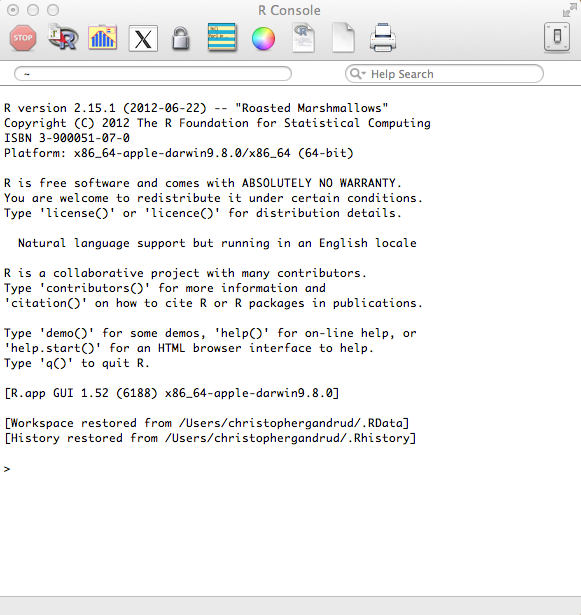
\includegraphics[scale=0.4]{/git_repositories/Rep-Res-Book/Source/Children/Chapter3/images3/BlankRConsole.png}
    \end{center}
\end{figure}

\subsection{Objects}\label{Objects}

If you've read a description of R before, you will probably have seen it referred to as an `object-oriented\index{object-oriented} language'.  What are objects? Objects are like the R language's nouns. They are things, like a vector of numbers, a data set, a word, a table of results from some analysis, and so on. Saying that R is `object-oriented' just means that R is focused on doing actions to objects. We will talk about the actions--commands and functions--later in this section. For now let's create a few objects.

\paragraph{Numeric \& string objects}

Objects can have a number of different data types. Let's make two simple objects. The first is a numeric type object. The other is a character object. We can choose almost any name we want for our objects as long as it begins with an alphabetic character and does not contain spaces.\footnote{It is common for people to use either periods (\texttt{.}) or capital letters (referred to as CamelBack) to separate words in object names instead of using spaces. For example: {\emph{new.data}} or {\emph{NewData}} rather than {\emph{new data}}.} Let's call our numeric object {\emph{Number}}. It is a good idea to give each object a different name. Also make sure that object names are different from variable names. This will avoid many complications like accidentally overwriting an object or confusing R about what object or component you are referring to.

To put something into the object we use the assignment operator\index{assignment operator}\footnote{The assignment operator is sometimes also referred to as the `gets arrow'.}: {\tt{\textless -}}. Let's assign the number 10 to our {\emph{Number}} object.

\begin{knitrout}
\definecolor{shadecolor}{rgb}{0.969, 0.969, 0.969}\color{fgcolor}\begin{kframe}
\begin{alltt}
Number <- 10
\end{alltt}
\end{kframe}
\end{knitrout}


\noindent To see the contents of our object, type its name.

\begin{knitrout}
\definecolor{shadecolor}{rgb}{0.969, 0.969, 0.969}\color{fgcolor}\begin{kframe}
\begin{alltt}
Number
\end{alltt}
\begin{verbatim}
## [1] 10
\end{verbatim}
\end{kframe}
\end{knitrout}


\noindent Lets's briefly breakdown this output. \texttt{10} is clearly the contents of {\emph{Number}}. The double hash (\texttt{\#\#}) is included to tell you that this is output rather than R code.\footnote{The double hash is generated automatically by {\emph{knitr}}. It makes easier to copy and past code into R from a presentation document by {\emph{knitr}}.} If you type the commands in your R Console, you will not get the double hash in your output. Finally, \texttt{[1]} is the row number of the object that 10 is on. Clearly our object only has one row.   

Creating a character object is very similar. The only difference is that you enclose the character string (letters in a word for example) inside of quotation marks ({\tt{""}}). To create an object called {\emph{Words}} that contains the character string ``Hello World".\label{StringObject}

\begin{knitrout}
\definecolor{shadecolor}{rgb}{0.969, 0.969, 0.969}\color{fgcolor}\begin{kframe}
\begin{alltt}
Words <- \hlstring{"Hello World"}
\end{alltt}
\end{kframe}
\end{knitrout}



An object's type is important to keep in mind as it determines what we can do to it. For example, you cannot take the mean of a character object like the {\emph{Words}} object we created earlier:

\begin{knitrout}
\definecolor{shadecolor}{rgb}{0.969, 0.969, 0.969}\color{fgcolor}\begin{kframe}
\begin{alltt}
\hlfunctioncall{mean}(Words)
\end{alltt}


{\ttfamily\noindent\textcolor{warningcolor}{\#\# Warning: argument is not numeric or logical: returning NA}}\begin{verbatim}
## [1] NA
\end{verbatim}
\end{kframe}
\end{knitrout}


\noindent Trying to find the mean of our {\emph{Words}} object gave us a warning message and returned the value {\tt{NA}}\index{NA}: not applicable. You can also think of {\tt{NA}} as meaning missing. To find out what type of object you have use the {\tt{class}} command. For example:

\begin{knitrout}
\definecolor{shadecolor}{rgb}{0.969, 0.969, 0.969}\color{fgcolor}\begin{kframe}
\begin{alltt}
\hlfunctioncall{class}(Words)
\end{alltt}
\begin{verbatim}
## [1] "character"
\end{verbatim}
\end{kframe}
\end{knitrout}


\paragraph{Vector \& data frame objects}

So far we have only looked at objects with a single number or character string.\footnote{These might be called scalar objects, though in R scalars are just vectors with a length of 1.} Clearly we often want to use objects that have many strings and numbers. In R these are usually data frame\index{data frame} type objects and are roughly equivalent the data structures you would be familiar with from using a program such as Microsoft Excel. We will be using data frames extensively throughout the book. Before looking at data frames it is useful to first look at the simpler objects that make up data frames. These are called vectors. Vectors are R's ``workhorse" \cite[]{Matloff2011}. Knowing how to use vectors\index{vector} will be especially helpful when you clean up raw data in Chapter \ref{DataClean} and make tables in Chapter \ref{TablesChapter}.\footnote{If you want information about other types of R objects such as lists\index{list} and matrices\index{matrix}, Chapter 1 of Norman Matloff's \citeyearpar{Matloff2011} book is a really good place to look.} \\[0.25cm]

\noindent {\bf{Vectors}} \\[0.25cm] Vectors are the ``fundamental data type" in R \cite[]{Matloff2011}. They are simply an ordered group of numbers, character strings, and so on.\footnote{In a vector every member of the group must be of the same type. If you want an ordered group of values with different types you can use lists\index{lists}.} It may be useful to think of basically all R objects as composed of vectors. For example, data frames are basically multiple vectors of the same length--i.e. they have the same number of rows--attached together to form columns. 

Let's create a simple numeric vector containing the numbers 2.8, 2, and 14.8. To do this we will use the \texttt{c} (concatenate)\index{concatenate} function:

\begin{knitrout}
\definecolor{shadecolor}{rgb}{0.969, 0.969, 0.969}\color{fgcolor}\begin{kframe}
\begin{alltt}
NumericVect <- \hlfunctioncall{c}(2.8, 2, 14.8)

\hlcomment{# Show NumericVect's contents}
NumericVect
\end{alltt}
\begin{verbatim}
## [1]  2.8  2.0 14.8
\end{verbatim}
\end{kframe}
\end{knitrout}


Vectors of character strings are created in a similar way. The only major difference is that each character string is enclosed in quotation marks like this:

\begin{knitrout}
\definecolor{shadecolor}{rgb}{0.969, 0.969, 0.969}\color{fgcolor}\begin{kframe}
\begin{alltt}
CharacterVect <- \hlfunctioncall{c}(\hlstring{"Albania"}, \hlstring{"Botswana"}, \hlstring{"Cambodia"})

\hlcomment{# Show CharacterVect's contents}
CharacterVect
\end{alltt}
\begin{verbatim}
## [1] "Albania"  "Botswana" "Cambodia"
\end{verbatim}
\end{kframe}
\end{knitrout}


To give you a preview of what we are going to do when we start working with real data sets, lets combine the two vectors {\emph{NumericVect}} and {\emph{CharacterVect}} into a new object with the \texttt{cbind}\index{cbind} function. This function binds the two vectors together side-by-side as columns.\footnote{If you want to combine objects as if they were rows of the same column(s) use the \texttt{rbind} function.}

\begin{knitrout}
\definecolor{shadecolor}{rgb}{0.969, 0.969, 0.969}\color{fgcolor}\begin{kframe}
\begin{alltt}
StringNumObject <- \hlfunctioncall{cbind}(CharacterVect, NumericVect)

\hlcomment{# Show StringNumObject's contents}
StringNumObject
\end{alltt}
\begin{verbatim}
##      CharacterVect NumericVect
## [1,] "Albania"     "2.8"      
## [2,] "Botswana"    "2"        
## [3,] "Cambodia"    "14.8"
\end{verbatim}
\end{kframe}
\end{knitrout}


\noindent By binding these two objects together we've created a new matrix\index{matrix} object.\footnote{Matrices are vectors with columns as well as rows.} You can see that the numbers in the {\emph{NumericVect}} column are between quotation marks. Matrices, like vectors can only have one data type. \\[0.25cm]

\noindent {\bf{Data frames}}

If we want to have an object with rows and columns and allow the columns to contain data with different types, we need to use data frames\index{data frame}. Let's use the \texttt{data.frame} command to combine the {\emph{NumericVect}} and {\emph{CharacterVect}} objects.

\begin{knitrout}
\definecolor{shadecolor}{rgb}{0.969, 0.969, 0.969}\color{fgcolor}\begin{kframe}
\begin{alltt}
StringNumObject <- \hlfunctioncall{data.frame}(CharacterVect, NumericVect)

\hlcomment{# Display contents of StringNumObject data frame}
StringNumObject
\end{alltt}
\begin{verbatim}
##   CharacterVect NumericVect
## 1       Albania         2.8
## 2      Botswana         2.0
## 3      Cambodia        14.8
\end{verbatim}
\end{kframe}
\end{knitrout}


\noindent There are two important things to notice in this output. The first is that because we used the same name for the data frame object as the previous matrix object, R deleted the matrix object and replaced it with the data frame. This is something to keep in mind when you are creating new objects. You will also notice that the strings in the {\emph{CharacterVect}} object are no longer in quotation marks. This does not mean that they are somehow now numeric data. To prove this try to find the mean of {\emph{CharacterVect}} by running it through the \texttt{mean}\index{mean} command:

\begin{knitrout}
\definecolor{shadecolor}{rgb}{0.969, 0.969, 0.969}\color{fgcolor}\begin{kframe}
\begin{alltt}
\hlfunctioncall{mean}(StringNumObject$ChacterVect)
\end{alltt}


{\ttfamily\noindent\textcolor{warningcolor}{\#\# Warning: argument is not numeric or logical: returning NA}}\begin{verbatim}
## [1] NA
\end{verbatim}
\end{kframe}
\end{knitrout}


\subsection{Component Selection}

The last bit of code will probably be confusing. Why do we have a dollar sign (\texttt{\$}) inbetween the name of our data frame object and the {\emph{CharcterVect}} vector? The dollar sign is called the component selector\index{component selection}.\footnote{It's also known as the element name operator.} It basically extracts a part of an object. In the previous example it extracted the {\emph{CharacterVect}} column from the {\emph{StringNumObject}} and fed it to the \texttt{mean} command, which tried (in this case unsuccessfully) to find its mean.

We can of course use the component selector to create new objects with parts of other objects. Imagine that we have the {\emph{StringNumObject}} and want an object with only the information in the numbers column. Let's use the following code:

\begin{knitrout}
\definecolor{shadecolor}{rgb}{0.969, 0.969, 0.969}\color{fgcolor}\begin{kframe}
\begin{alltt}
NewNumeric <- StringNumObject$NumericVect

\hlcomment{# Display contents of NewNumeric}
NewNumeric
\end{alltt}
\begin{verbatim}
## [1]  2.8  2.0 14.8
\end{verbatim}
\end{kframe}
\end{knitrout}


\noindent Knowing how to use the component selector will be especially useful when we discuss making tables for presentation documents in Chapter \ref{TablesChapter}.

Using the component selector can lead to long repetitive code. You have to write the object name, a dollar sign, and the component name every time you want to select a component. You can streamline your code by using commands such as \texttt{attach}\index{attach} and \texttt{with}\index{with}. For examples in this book I largely avoid using these commands. I generally use the component selector. Though it creates longer code, I find code written with the component selector is easier to follow. It's always clear which object we are selecting a component from. \todo{Add with and attach discussion.}

\subsection{Subscripts}

Another way to select parts of an object is to use subscripts\index{subscripts}. You have already seen subscripts in the output from our examples so far. They are denoted with square braces (\texttt{[]}). We can use subscripts to select not only columns from data frames but also rows and individual cells. As we began to see in some of the previous output, each part of a data frame has an address captured by its row and column number. We can tell R to find a part of an object by putting the row number/name, column number/name, or both in square braces. The first part denotes the rows and separated by a comma (\texttt{,}) are the columns. 

To give you an idea of how this works lets use the {\emph{cars}} data set that comes with R. Use the \texttt{head} command to get a sense of what this data set looks like.

\begin{knitrout}
\definecolor{shadecolor}{rgb}{0.969, 0.969, 0.969}\color{fgcolor}\begin{kframe}
\begin{alltt}
\hlfunctioncall{head}(cars)
\end{alltt}
\begin{verbatim}
##   speed dist
## 1     4    2
## 2     4   10
## 3     7    4
## 4     7   22
## 5     8   16
## 6     9   10
\end{verbatim}
\end{kframe}
\end{knitrout}


\noindent We can see a data frame with information on various cars speeds ({\emph{speed}}) and stopping distances ({\emph{dist}}). If we want to select only the third through seventh rows we can use the following subscript commands:

\begin{knitrout}
\definecolor{shadecolor}{rgb}{0.969, 0.969, 0.969}\color{fgcolor}\begin{kframe}
\begin{alltt}
cars[3:7, ]
\end{alltt}
\begin{verbatim}
##   speed dist
## 3     7    4
## 4     7   22
## 5     8   16
## 6     9   10
## 7    10   18
\end{verbatim}
\end{kframe}
\end{knitrout}


\noindent The colon (\texttt{:}) creates a sequence of whole numbers from 3 to 7. To select the fourth row of the {\emph{dist}} column we can type:

\begin{knitrout}
\definecolor{shadecolor}{rgb}{0.969, 0.969, 0.969}\color{fgcolor}\begin{kframe}
\begin{alltt}
cars[4, 2]
\end{alltt}
\begin{verbatim}
## [1] 22
\end{verbatim}
\end{kframe}
\end{knitrout}


\noindent An equivalent way to do this is:

\begin{knitrout}
\definecolor{shadecolor}{rgb}{0.969, 0.969, 0.969}\color{fgcolor}\begin{kframe}
\begin{alltt}
cars[4, \hlstring{"dist"}]
\end{alltt}
\begin{verbatim}
## [1] 22
\end{verbatim}
\end{kframe}
\end{knitrout}


\noindent Finally, we can even include a vector of column names to select:

\begin{knitrout}
\definecolor{shadecolor}{rgb}{0.969, 0.969, 0.969}\color{fgcolor}\begin{kframe}
\begin{alltt}
cars[4, \hlfunctioncall{c}(\hlstring{"speed"}, \hlstring{"dist"})]
\end{alltt}
\begin{verbatim}
##   speed dist
## 4     7   22
\end{verbatim}
\end{kframe}
\end{knitrout}


\subsection{Functions and commands}

If objects are the nouns of the R language, functions and commands\footnote{For the purposes of this book I treat the two as the same.} are the verbs. They do things to objects. Let's use the \texttt{mean} command as an example. This command takes the mean of a numeric vector object. Remember our {\emph{NumericVect}} object from before:

\begin{knitrout}
\definecolor{shadecolor}{rgb}{0.969, 0.969, 0.969}\color{fgcolor}\begin{kframe}
\begin{alltt}
\hlcomment{# Show contents of NumericVect}
NumericVect
\end{alltt}
\begin{verbatim}
## [1]  2.8  2.0 14.8
\end{verbatim}
\end{kframe}
\end{knitrout}


\noindent To find the mean of this object simply type:

\begin{knitrout}
\definecolor{shadecolor}{rgb}{0.969, 0.969, 0.969}\color{fgcolor}\begin{kframe}
\begin{alltt}
\hlfunctioncall{mean}(x = NumericVect)
\end{alltt}
\begin{verbatim}
## [1] 6.533
\end{verbatim}
\end{kframe}
\end{knitrout}


\noindent We use the assignment operator to place a command's output into an object. For example,

\begin{knitrout}
\definecolor{shadecolor}{rgb}{0.969, 0.969, 0.969}\color{fgcolor}\begin{kframe}
\begin{alltt}
MeanNumericVect <- \hlfunctioncall{mean}(x = NumericVect)
\end{alltt}
\end{kframe}
\end{knitrout}


\noindent Notice that we typed the command's name then enclosed the object name in parentheses immediately afterwards. This is the basic sytax that all commands use, i.e. \texttt{COMMAND(ARGUMENTS)}. If you don't want to explicitly include an argument you still need to type the parentheses after the command. 

\subsection{Arguments}

Arguments\index{argument} modify what commands do. In our most recent example we gave the \texttt{mean} command one argument (\texttt{x = NumericVect}) telling it that we wanted to find the mean of {\emph{NumericVect}}. Arguments use the \texttt{ARGUMENTLABEL = VALUE} syntax.\footnote{Note: you do not have to put spaces between the argument label and the equals sign or the equals sign and the value. However, having spaces can make your code easier for other people to read.} 

To find all of the arguments that an argument can accept look at the {\bf{Arguments}} section of the command's help file\index{help file}. To access the help file type: \texttt{?COMMAND}. For example,

\begin{knitrout}
\definecolor{shadecolor}{rgb}{0.969, 0.969, 0.969}\color{fgcolor}\begin{kframe}
\begin{alltt}
?mean
\end{alltt}
\end{kframe}
\end{knitrout}


\noindent The help file will also tell you the default values that the arguments are set to. Clearly, you do not need to explicitly set an argument if you want to use it's default value.

You have to fairly precise with the syntax for your argument's values. Arguments for logical arguments must written as \texttt{TRUE} or \texttt{FALSE}.\footnote{They can be abbreviated \texttt{T} and \texttt{F}.} Arguments that are character strings should be in quotation marks.

Let's see how to use multiple arguments with the \texttt{round} command. This command rounds a vector of numbers. We can use the \texttt{digits} option to specify how many decimal places we want the numbers rounded to. To round the object \emph{MeanNumericVect} to one decimal place type:

\begin{knitrout}
\definecolor{shadecolor}{rgb}{0.969, 0.969, 0.969}\color{fgcolor}\begin{kframe}
\begin{alltt}
\hlfunctioncall{round}(x = MeanNumericVect, digits = 1)
\end{alltt}
\begin{verbatim}
## [1] 6.5
\end{verbatim}
\end{kframe}
\end{knitrout}


\noindent You can see that arguments are separated by commas. 

Some arguments do not need to be explicitly labelled. For example we could have written:

\begin{knitrout}
\definecolor{shadecolor}{rgb}{0.969, 0.969, 0.969}\color{fgcolor}\begin{kframe}
\begin{alltt}
\hlcomment{# Find mean of NumericVect}
\hlfunctioncall{mean}(NumericVect)
\end{alltt}
\begin{verbatim}
## [1] 6.533
\end{verbatim}
\end{kframe}
\end{knitrout}


\noindent R will do its best to figure out what you want and will only give up when it can't. This will generate an error message. However, to avoid any misunderstandings between yourself and R it can be good practice to label all of your arguments. This will also make your code easier for other people to read, i.e. it will be more reproducible.

Finally, you can stack arguments inside of other arguments. To have R find the mean of {\emph{NumericVect}} and round it to one decimal place use:

\begin{knitrout}
\definecolor{shadecolor}{rgb}{0.969, 0.969, 0.969}\color{fgcolor}\begin{kframe}
\begin{alltt}
\hlfunctioncall{round}(\hlfunctioncall{mean}(NumericVect), digits = 1)
\end{alltt}
\begin{verbatim}
## [1] 6.5
\end{verbatim}
\end{kframe}
\end{knitrout}


\subsection{The Workspace \& History}

All of the objects you create become part of your workspace\index{workspace}. Use the \texttt{ls}\index{ls} command to list all of the objects in your current workspace.\footnote{Note: your workspace will probably include different objects than this example. These are all of the objects created to knit the book up to this point.}

\begin{knitrout}
\definecolor{shadecolor}{rgb}{0.969, 0.969, 0.969}\color{fgcolor}\begin{kframe}
\begin{alltt}
\hlfunctioncall{ls}()
\end{alltt}
\begin{verbatim}
##  [1] "AgMethaneData"   "CharacterVect"   "Data"           
##  [4] "DataUrl"         "doInstall"       "MeanNumericVect"
##  [7] "NBModel"         "NBModelSum"      "NBSumDataFrame" 
## [10] "NBTable"         "NewNumeric"      "Number"         
## [13] "NumericVect"     "StringNumObject" "temp"           
## [16] "toInstall"       "url"             "UrlAddress"     
## [19] "Words"
\end{verbatim}
\end{kframe}
\end{knitrout}


To save the workspace into an \texttt{.RData} file use the \texttt{save.image}\index{save.image} command. The main argument of the \texttt{save.image} command is the file path you would like the file saved into. If you don't specify the file path it will save in your current working directory (see Chapter \ref{DirectoriesChapter}). 

You should generally avoid saving your workspace. Instead, when you return to working on a project rerun the source code files. This avoids any complications caused when you use an object in your workspace that is left over from running an older version of the source code.\footnote{For example, imagine you create an object, then change the source code you used to create the object. However, there is a syntax error in the new version of the source code. The old object won't be overwritten and you will be mistakenly using the old object in future commands.} The only time when saving your workspace is very useful is when it includes an object that was computationally difficult and took a long time to create. In this case it is still useful to clean up the workspace before saving it by using the \texttt{rm} command\index{rm} to remove the other objects. For example, to remove the \texttt{CharacterVect} and \texttt{Words} objects type:

\begin{knitrout}
\definecolor{shadecolor}{rgb}{0.969, 0.969, 0.969}\color{fgcolor}\begin{kframe}
\begin{alltt}
\hlfunctioncall{rm}(CharacterVect, Words)
\end{alltt}
\end{kframe}
\end{knitrout}


When you enter a command into R they become part of your history. To see the most recent commands in your history use the \texttt(history) command. You can also use the up and down arrows on your keyboard when your cursor is in the R console to scroll through your history.

\subsection{Installing new libraries and loading commands}\label{Packages}

Commands are stored in R libraries\index{R libraries}. R automatically loads a number of basic libraries by default. One of the great things about R is the many user-created libraries\footnote{For the latest list see: \url{http://cran.r-project.org/web/packages/available_packages_by_name.html}} that greatly expand the number of commands we can use. To install commands that do not come with base R you need to install the add-on packages\index{packages}\label{packages} that contain them. To do this use the {\tt{install.packages}}\index{install.packages} command. By default this command downloads and installs the packages from the Comprehensive R Archive Network (CRAN)\index{CRAN}. 

For the code you need to install all of the package libraries used in this book see page \pageref{ReqPackages}. When you install a package, you will likely be given a list of mirrors\index{mirrors, CRAN} from which you can download the package. Simply select the mirror closest to you.

Once you have installed a package you need to load it so that you can use its functions. Use the \texttt{library} command to load a package library. Use the following code to load the {\emph{ggplot2}} library that we use in Chapter \ref{FiguresChapter} to create figures.

\begin{knitrout}
\definecolor{shadecolor}{rgb}{0.969, 0.969, 0.969}\color{fgcolor}\begin{kframe}
\begin{alltt}
\hlfunctioncall{library}(ggplot2)
\end{alltt}
\end{kframe}
\end{knitrout}


\noindent Please note for the examples in this book I only specify the library a command is in if the library is not loaded by default when you start an R session. 

%%%%%%%%%%%%%%% Using RStudio
\section{Using RStudio}

As I mentioned in Chapter \ref{Intro}, RStudio is an integrated development environment for R. It provides a centralized and well organized place to do almost anything you want to do with R. As we will see later in this chapter, it is especially well integrated with literate programming tools for reproducible research. Right now let's take a quick tour of the basic RStudio window.

\paragraph{The default window}

When you first open RStudio\index{RStudio} you should see a default window that looks like Figure \ref{BlankMain}. In this figure you see three window panes\index{RStudio pane}. The large one on the left is the {\emph{Console}}. This pane functions exactly the same as the console in regular R. Other panes include the {\emph{Workspace/History}} panes, usually in the upper right-hand corner. The Workspace pane shows you all of the objects in your current workspace and some of their characteristics, like how many observations a data frame has. You can click on an object in this pane to see its contents. This is especially useful for quickly looking at a data set in much the same way that you can visually scan a Microsoft Excel spreadsheet. The History pane records all of the commands you have run. It allows you to rerun code and insert it into a source code file.

\begin{figure}[ht]
    \caption{RStudio Startup Panel}
    \label{BlankMain}
    \begin{center}
    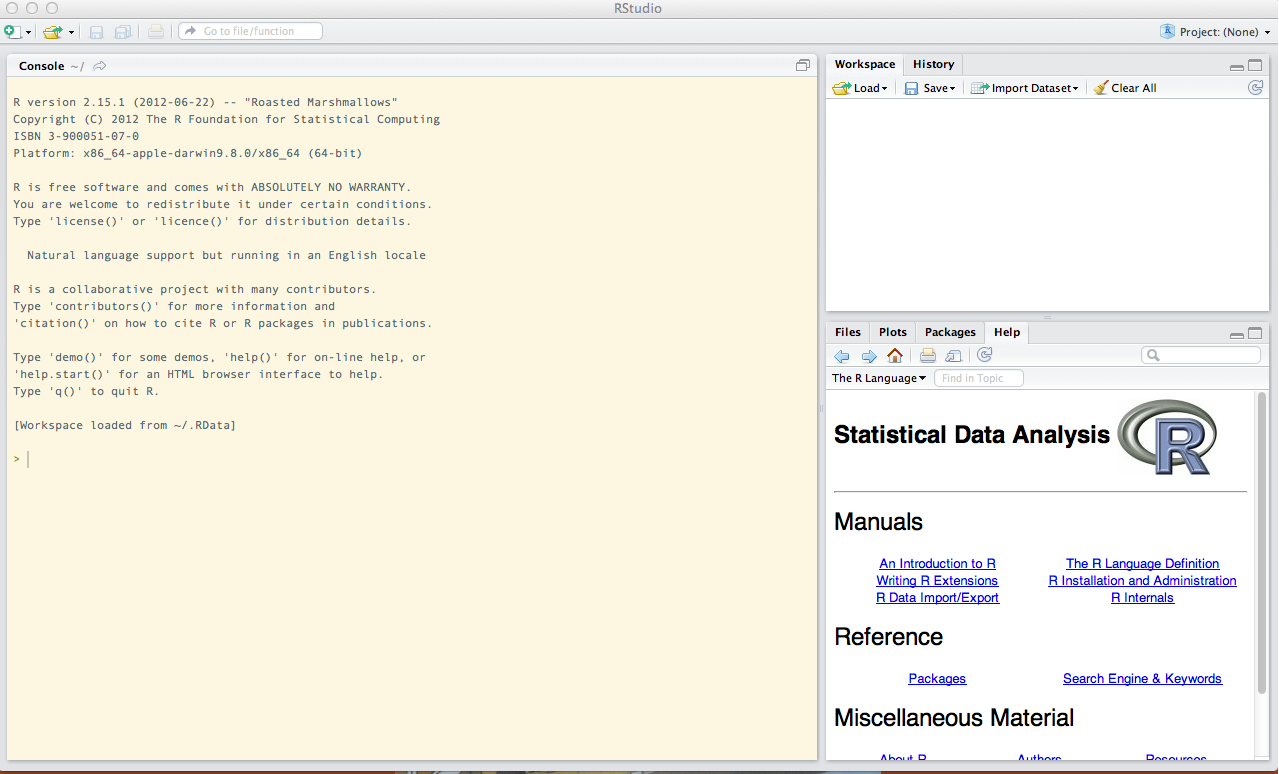
\includegraphics[width = \textwidth]{/git_repositories/Rep-Res-Book/Source/Children/Chapter3/images3/BlankMainPanel.png}
    \end{center}
\end{figure}

In the lower right-hand corner you will see the {\emph{Files/Plots/Packages/Help}} pane. We will discuss the Files pane in more detail in Chapter \ref{DirectoriesChapter}. Basically, it allows you to see and organize your files. The Plots pane is where figures you create in R appear. This pane allows you to see all of the figures you have created in a session using the right and left arrow icons. It also lets you save the figures in a variety of formats. The Packages pane shows the packages you have installed, allows you to load individual packages by clicking on the dialog box next to them, access their manual files (click on the package name), update the packages, and even install new packages. Finally, the Help pane shows you help files. You can search for help files and search within help files using this pane.  

\paragraph{The source pane}

There is an important pane that does not show up when you open RStudio for the first time. This is the {\emph{Source}} pane. The Source pane is where you create, edit, and run your source code files. It also functions as an editor for your markup files. It is the center of reproducible research in RStudio. Let's first look at how to use the Source pane with regular R files. We will cover how to use the Source pane with literate programming file formats--e.g. R Markdown and R LaTeX--in more detail after first discussing the {\emph{knitr}} basics in the next section. 

R source code files have the file extension \texttt{.R}. You can create a new source code document, which will open a new Source pane, by going to the menu bar and clicking on \texttt{File} \textrightarrow \: \texttt{New}. In this drop down menu you have the option to create a variety of different source code documents. Select the \texttt{R Source} option. You should now see a new pane with a bar across the top that looks like the first image in Figure \ref{SourcePanes}. To run the R code you have in your source code file simply highlight it\footnote{If you are only running one line of code you don't need to highlight the code, you can simply put your cursor on that line.} and click the \texttt{Run} icon on the top bar. This sends the code to the console where it is executed. The icon to the right of \texttt{Run} simply runs the code above where you have highlighted. The \texttt{Source} icon next to this runs all of the code in the file using R's \texttt{source} command\index{source command}. The icon next to \texttt{Source} is for compiling RStudio Notebooks\index{RStudio Notebook}. We will look at RStudio Notebooks later in this chapter.

\begin{figure}[ht]
    \caption{RStudio Source Code Pane Top Bars}
    \label{SourcePanes}
    \begin{center}
    
        \begin{subfigure}
            \caption{R Source Code}
            
\includegraphics[width = \textwidth]{/git_repositories/Rep-Res-Book/Source/Children/Chapter3/images3/RSourceBar.png}
        \end{subfigure}
        \vspace{0.5cm}
        
        \begin{subfigure}
            \caption{R Markdown Files}
            
\includegraphics[width = \textwidth]{/git_repositories/Rep-Res-Book/Source/Children/Chapter3/images3/MarkdownSourceBar.png}
        \end{subfigure}
        \vspace{0.5cm}
        
        \begin{subfigure}
            \caption{LaTeX Markdown Files}
            
\includegraphics[width = \textwidth]{/git_repositories/Rep-Res-Book/Source/Children/Chapter3/images3/LaTeXSourceBar.png}
        \end{subfigure}
        
    \end{center}
\end{figure}



%%%%%%%%%%%%% Using knitr
\section{Using knitr: the basics}

To get started with {\emph{knitr}}\index{knitr} in R or RStudio we need to learn some of the basic concepts and syntax. The concepts are the same regardless of the markup language we are knitting R code with, but much of the syntax varies by markup language.

\subsection{File extensions}

When you save a knitable file use a file extension that indicates (a) that it is knitable and (b) what markup language it is using. You can use a number of file extensions for R Markdown files including: \texttt{.Rmd} and \texttt{.Rmarkdown}. LaTeX documents that include {\emph{knitr}} code chunks are generally called R Sweave\index{R Sweave} files and have the file extension {\tt{.Rnw}}. This terminology is a little confusing. It is a holdover from {\emph{knitr}}'s main literate programming predecessor {\emph{Sweave}} \cite[]{Leisch2002}. You can also use the less confusing file extension \texttt{.Rtex}, as regular LaTeX files have the extension \texttt{.tex}. However, the syntax for \texttt{.Rtex} files is different from that used with \texttt{.Rnw} files. We'll look at this issue in more detail below.

\subsection{Code Chunks}

When you want to include R code into your markup presentation documents, place them in a code chunk\index{code chunk}. Code chunk syntax differs depending on the markup language we are using to write our documents. Let's see the syntax for R Markdown and R LaTeX files.

\paragraph{R Markdown}

In R Markdown files we begin a code chunk by writing the head: \texttt{\`\`\`\\ \{r\} }. A code chunk is closed--ended--simply with: \`\`\`\ . For example:

\begin{knitrout}
\definecolor{shadecolor}{rgb}{0.969, 0.969, 0.969}\color{fgcolor}\begin{kframe}
\begin{alltt}
```\{r\}
\hlcomment{# Example of a R Markdown code chunk}
StringNumObject <- \hlfunctioncall{cbind}(CharacterVect, NumericVect)
```
\end{alltt}
\end{kframe}
\end{knitrout}


\paragraph{R LaTeX}

There are two different ways to delimit code chunks in R LaTeX documents. One way largely emulates the established {\emph{Sweave}} syntax.\footnote{The syntax has its genesis in a literate programming tool called noweb \cite[]{Leisch2002,RamseyNoweb}.} {\emph{Knitr}} also supports files with the {\tt{.Rtex}} extension, though the code chunk syntax is different. I will cover both types of syntax for code chunks in LaTeX documents. Throughout the book I use the older and more established {\emph{Sweave}} style syntax. \\[0.25cm]

\noindent {\bf{Sweave-style}} \\[0.25cm]

Traditional Sweave-style code chunks begin with the following head: \texttt{\textless\textless \textgreater\textgreater=}. The code chunk is closed with an at sign (@).

\begin{knitrout}
    \definecolor{shadecolor}{rgb}{0.969, 0.969, 0.969}
    \color{fgcolor}\begin{kframe}
        \begin{alltt}
\textless\textless \textgreater\textgreater=
\hlcomment{# Example of a Sweave-style code chunk}
StringNumObject <- \hlfunctioncall{cbind}(CharacterVect, NumericVect)
@
        \end{alltt}
    \end{kframe}
\end{knitrout}

\noindent {\bf{Rtex-style}} \\[0.25cm]

Sweave-style code chunk syntax is fairly baroque compared to the Rtex-style syntax. To begin a code chunk in an \texttt{Rtex} file simply type double percent signs followed by \texttt{begin.rcode}, i.e. \texttt{\%\% begin.rcode}. To close the chunk you use double percent signs: \texttt{\%\%}. Each line in the code chunk needs to begin with a single percent sign. For example:

\begin{knitrout}
    \definecolor{shadecolor}{rgb}{0.969, 0.969, 0.969}
    \color{fgcolor}
    \begin{kframe}
        \begin{verbatim}
%% begin.rcode
% # Example of a Rtex-style code chunk
% StringNumObject <- cbind(CharacterVect, NumericVect)
%%
            \end{verbatim}
        \end{kframe}
\end{knitrout}

\paragraph{Code chunk labels}

Each chunk has a label. When a code chunk creates a plot or the output is cached\index{cache}--stored for future use--{\emph{knitr}} uses the chunk label for the new file's name. If you do not explicitly give the chunk a label it will be assigned one like: \texttt{unnamed-chunk-1}.

To explicitly assign chunk labels in R Markdown documents place the label name inside of the braces after the \texttt{r}. If we wanted to use the label \texttt{ChunkLabel} we would simply type:

\begin{knitrout}
\definecolor{shadecolor}{rgb}{0.969, 0.969, 0.969}\color{fgcolor}\begin{kframe}
\begin{alltt}
```\{r ChunkLabel\}
\hlcomment{# Example chunk label}
```
\end{alltt}
\end{kframe}
\end{knitrout}


\noindent The same general format applies to the two types of LaTeX chunks. In Sweave-style chunks we would type: \texttt{\textless\textless ChunkLabel\textgreater\textgreater=}. In Rtex-style we use: \texttt{\%\% begin.rcode ChunkLabel}.

Try not to use spaces or periods in your label names. Also remember that chunk labels {\emph{must}} be unique.

\paragraph{Code chunk options}

There are many times when we want to change how our code chunks are knitted and presented. Maybe we only want to show the code and not the results or perhaps we don't want to show the code at all but just a figure that it produces. Maybe we want the figure to be formatted on a page in a certain way. To make these changes, and many others we can specify code chunk options\index{code chunk options}.

Like chunk labels, you specify options in the chunk head. Place them after the chunk label, separated by a comma. Chunk options are written following pretty much the same rules as regular R command arguments. They have a similar \texttt{OPTIONLABEL=VALUE} structure as arguments. The option values must be written in the same way that argument values are. Character strings need to be inside of quotation marks. The logical \texttt{TRUE} and \texttt{FALSE} operators cannot be written ``true" and ``false". For example, imagine we have a Markdown code chunk called \texttt{ChunkLabel}. If we only want to have {\emph{knitr}} include the code in our document, but not actually run it we use the option \texttt{eval=FALSE}. This option tells {\emph{knitr}} not to evaluate (run) the code chunk.

\begin{knitrout}
\definecolor{shadecolor}{rgb}{0.969, 0.969, 0.969}\color{fgcolor}\begin{kframe}
\begin{alltt}
```\{r ChunkLabel, eval=FALSE\}
\hlcomment{# Example of a non-evaluated code chunk}
StringNumObject <- \hlfunctioncall{cbind}(CharacterVect, NumericVect)
```
\end{alltt}
\end{kframe}
\end{knitrout}


\noindent Note that all labels and code chunk options must be on the same line. Options are separated by commas. The syntax for {\emph{knitr}} options is the same regardless of the markup language. Here is the same chunk option in Rtex-style syntax:

\begin{knitrout}
    \definecolor{shadecolor}{rgb}{0.969, 0.969, 0.969}
    \color{fgcolor}
    \begin{kframe}
        \begin{verbatim}
%% begin.rcode ChunkLabel, eval=FALSE
% # Example of a non-evaluated code chunk
% StringNumObject <- cbind(CharacterVect, NumericVect)
%%
            \end{verbatim}
        \end{kframe}
\end{knitrout}

Throughout this book we will look at a number of different code chunk options. All of the chunk options we will use in this book are listed in Table \ref{ChunkOptionsTable}. For the full list of {\emph{knitr}} options see the {\emph{knitr}} chunk options page maintained by {\emph{knitr}}'s creator Yihui Xie: \url{http://yihui.name/knitr/options#package_options}.\todo{Note: this table will be expanded as the later chapters are expanded.} 


\begin{table}
  \caption{A Selection of {\emph{knitr}} Code Chunk Options}
  \begin{center}
  \label{ChunkOptionsTable}
  \begin{tabular}{l c p{5cm}}
    \hline  
    Chunk Option Label & Type & Description \\[0.25cm] \hline\hline
    \texttt{eval} & Logical & Whether or not to run the chunk. \\[0.25cm]
    \texttt{echo} & Logical & Whether or not to include the code in the presentation document. \\[0.25cm]
    \texttt{error} & Logical & Whether or not to include errors. \\[0.25cm]
    \texttt{engine} & Character & Set the programming language for {\emph{knitr}} to evaluate the code chunk with. \\[0.25cm]
    \texttt{fig.align} & Character & Aligns figures. \\[0.25cm]
    \texttt{fig.height} & Numeric & Sets figures' height. \\[0.25cm]
    \texttt{fig.width} & Numeric & Sets figures' width. \\[0.25cm]
    \texttt{include} & Logical & When \texttt{include=FALSE} the chunk is evaluated, but the results are not included in the presentation document. \\[0.25cm]
    \texttt{message} & Logical & Whether or not to include message messages. \\[0.25cm]
    \texttt{results} & Character & How to include results in the presentation document. \\[0.25cm]
    \texttt{warning} & Logical & Whether or not to include warnings. \\[0.25cm]
    \hline
  \end{tabular}
  \end{center}
\end{table}

\subsection{Global options}

So far we have only looked at how to set local options\index{local chunk options} in {\emph{knitr}} code chunks, i.e. options for only one specific chunk. If we want an option to apply to all of the chunks in our document we can set global chunk options\index{global chunk options}. Options are `global' in the sense that they apply to the entire document. Setting global chunk options helps us create documents that are formatted consistently without having to repetitively specify the same option every time we create a new code chunk. For example, in this book I center almost all of the the figures. Instead of using the \verb|fig.align='center'| option in each code chunk that creates a figure, I set the option globally.

To set a global option first create a new code chunk at the beginning of your document\footnote{In Markdown, you can put global chunk options at the very top of the document. In LaTeX they should be placed after the \texttt{\textbackslash{}begin\{document\}} command (see Chapter \ref{LatexChapter} for more information on how LaTeX documents are structured).} You will probably want to set the option {\tt{echo=FALSE}} so that {\emph{knitr}} doesn't echo the code. Inside the code chunk use {\tt{opts\_chunk\$set}}. You can set any chunk option as an argument to {\tt{opts\_chunk\$set}}. The option will be applied across your document, unless you set a different local option. 

Here is an example of how you can center align all of the figures in a Markdown document created {\emph{knitr}} code chunks. Place the following code at the beginning of the document:

\begin{knitrout}
    \definecolor{shadecolor}{rgb}{0.969, 0.969, 0.969}
    \color{fgcolor}
    \begin{kframe}
        \begin{alltt}
\textless{\textless}ChunkLabel\textgreater{\textgreater}=
# Center align all knitr figures
opts_chunk$set(fig.align='center')
@
        \end{alltt}
    \end{kframe}
\end{knitrout}

\subsection{knitr package options}

{\emph{Knitr}} package options\index{package options} affect how the package itself runs. For example, the {\tt{progress}} option can be set as either {\tt{TRUE}} or {\tt{FALSE}}\footnote{It's set as {\tt{TRUE}} by default.} depending on whether or not you want a progress bar\index{progress bar} to be displayed when you knit a code chunk.\footnote{The {\emph{knitr}} progress bar looks like this {\tt{|>>>>>>| 100\%}} and indicates how much of a code chunk has been run.} You can use {\tt{base.dir}} to set the directory where you want all of your figures to be saved to (see Chapter \ref{DirectoriesChapter}) or the {\tt{child.path}} option to specify where child documents are located (see Chapter \ref{LargeDocs}).

You set package options in a similar way as global chunk options with {\tt{opts\_knit\$set}}. For example, to turn off the progress bar when knitting documents include this code at the beginning of the document:

\begin{knitrout}
    \definecolor{shadecolor}{rgb}{0.969, 0.969, 0.969}
    \color{fgcolor}
        \begin{kframe}
            \begin{alltt}
\textless{\textless}ChunkLabel\textgreater{\textgreater}=
# Turn off knitr progress bar
opts_knit$set(progress=FALSE)
@
            \end{alltt}
        \end{kframe}
\end{knitrout}


\subsection{Hooks}

You can also set hooks\index{hooks}. Hooks come in two types: chunk hooks and output hooks. Chunk hooks\index{chunk hooks} run a function before or after a code chunk. Output hooks\index{output hooks} change how the raw output is formatted. I don't cover hooks in much detail in this book. For more information on hooks, please see Yihui Xie's webpage: \url{http://yihui.name/knitr/hooks}.

%%%%%%%%%% Knitr & RStudio
\subsection{knitr \& RStudio}

RStudio is highly integrated with {\emph{knitr}} and the markup languages knitr works with. Because of this integration it is easier to create and compile {\emph{knitr}} documents than doing so in plain R. Most of the RStudio/{\emph{knitr}} features are accessed in the Source pane\index{Source pane}. The Source pane's appearance and capabilities change depending on the type of file you have open in it. RStudio uses a file's extension\index{file extension} to determine what type of file you have open.\footnote{You can manually set how you want the Source pane to act by selecting the file type using the drop down menu in the lower right-hand corner of the Source pane.} We have already seen some of the features the Source pane has for R source code files. Let's now look at how to use {\emph{knitr}} with R source code files as well as the markup formats we cover in this book: R Markdown\index{R Markdown}, and R LaTeX\index{R LaTeX}. \\[0.25cm]

\paragraph{Compiling R source code notebooks}

If you want a quick well formatted account of the code that you ran and the results that you got you can use RStudio's ``Compile Notebook"\index{notebook} capabilities. RStudio uses {\emph{knitr}} to create a standalone HTML file that includes all of the code from an R source file as well as the output. This can be useful for recording the steps you took to do an analysis. You can see an example RStudio Notebook in Figure \ref{NotebookExample}. 

If you want to create a Notebook from an open R source code file simply click the \texttt{Compile Notebook} icon in the Source pane's top bar (see Figure \ref{SourcePanes}).\footnote{Alternatively, \texttt{File} \textrightarrow \; \texttt{Compile Notebook\ldots}} Then click the \texttt{Compile} button in the window that pops up. In Figure \ref{NotebookExample} you can see near the top center right a small globe icon next to the word ``Publish". Clicking this allows you to publish your Notebook to RPubs (\url{http://www.rpubs.com/}). RPubs is a site for sharing your Notebooks over the internet. You can publish not only Notebooks, but also any {\emph{knitr}} Markdown document you compile in RStudio.

\begin{figure}
    \caption{RStudio Notebook Example}
    \label{NotebookExample}
    \begin{center}
    
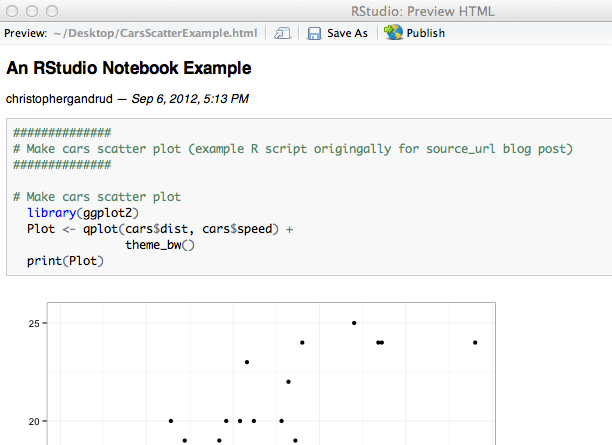
\includegraphics[scale=0.4]{/git_repositories/Rep-Res-Book/Source/Children/Chapter3/images3/NotebookExample.png}
    \end{center}
\end{figure}

\paragraph{R Markdown} The second image in figure \ref{SourcePanes} is what the Source pane's top bar looks like when you have an R Markdown file open. You'll notice the familiar \texttt{Run} button for running R code. At the far right you can see a new \texttt{Chunks} drop down menu. In this menu you can select \texttt{Insert Chunk} to insert the basic syntax required for a code chunk. There is also an option to \texttt{Run Current Chunk}--i.e. the chunk where your cursor is located--\texttt{Run Next Chunk}, and \texttt{Run All} chunks. You can navigate to a specific chunk using a drop down menu on the bottom left-hand side of the Source pane (not shown). This can be very useful if you are working with a long document. To knit your file click the \texttt{Knit HTML} icon on the left side of the Source pane's top bar. This will create a knitted HTML file as well as a regular Markdown file with highlighted code, output, and figures in your R Markdown's directory. Other useful buttons in the R Markdown Source pane's top bar include the \texttt{ABC} spell check icon and \texttt{MD} icon, which gives you a Markdown syntax reference file in the Help pane.

Another useful RStudio {\emph{knitr}} integration feature is that RStudio can properly highlight both the markup language syntax and the R code in the Source pane. This makes your source code much easier to read and navigate. RStudio can also fold code chunks. This makes navigating through long documents, with long code chunks, much easier. In the first image in Figure \ref{CodeFold} you can see a small downward facing arrow at line 25. If you click this arrow the code chunk will collapse, like in the second image in Figure \ref{CodeFold}. To unfold the chunk, just click on the arrow again.

You may also notice that there are code folding arrows on lines 27 and 34 in the first image. These allow us to fold parts of the code chunk. To enable this option create a comment line with at least one hash before the comment text and at least four after it like this:

\begin{knitrout}
\definecolor{shadecolor}{rgb}{0.969, 0.969, 0.969}\color{fgcolor}\begin{kframe}
\begin{alltt}
\hlcomment{#### An RStudio Foldable Comment ####}
\end{alltt}
\end{kframe}
\end{knitrout}


\noindent You will be able to fold all of the text after this comment up until the next similarly formatted comment (or the end of the chunk).

\begin{figure}[ht!]
    \caption{Folding Code Chunks in RStudio}
    \label{CodeFold}
    \begin{center}
    \begin{subfigure}  
        \caption{Not Folded}   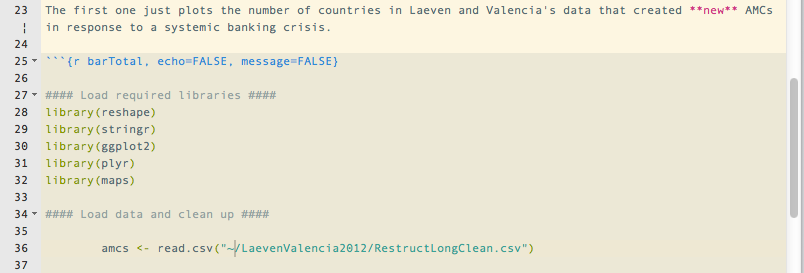
\includegraphics[width = \textwidth]{/git_repositories/Rep-Res-Book/Source/Children/Chapter3/images3/MarkdownNoCollapse.png}
    \end{subfigure} \\[0.5cm]
    
    \begin{subfigure}
        \caption{Folded}
      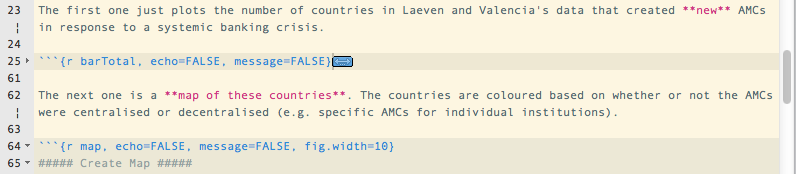
\includegraphics[width = \textwidth]{/git_repositories/Rep-Res-Book/Source/Children/Chapter3/images3/MarkdownCollapse.png}        
    \end{subfigure}
    \end{center}
\end{figure}

\paragraph{R LaTeX}

You can see in the final image in Figure \ref{SourcePanes} that many of the Source pane options for R LaTeX files are the same as R Markdown files. The key differences being that there is a \texttt{Compile PDF} icon instead of \texttt{Knit HTML}. Clicking this icon knits the file and creates a PDF file in your R LaTeX file's directory. There is also a \texttt{Format} icon instead of \texttt{MD}. This actually inserts LaTeX formatting commands into your document for things such as section headings and bullet lists. These commands can be very tedious to type out by hand.


\paragraph{Change default .Rnw knitter}

By default RStudio is set up to use Sweave\index{Sweave} for compiling LaTeX documents. To use {\emph{knitr}} instead of Sweave to knit \texttt{.Rnw} files you should click on \texttt{Tools} in the RStudio menu bar then click on \texttt{Options} window\index{RStudio Options window}. Once the {\bf{Options}} window opens, click on the \texttt{Sweave} button. Select \texttt{knitr} from the drop down menu for ``Weave files using:". Finally, click \texttt{Apply}.\footnote{In the Mac version of RStudio, you can also access the \texttt{Options} window via \texttt{RStudio} \textrightarrow \texttt{Preferences} in the menu bar.} 

\subsection{knitr \& R}

As {\emph{knitr}} is a regular R package, you can of course knit documents in R (or using the console in RStudio). All of the {\emph{knitr}} syntax in your markup document is the same as before, but instead of clicking a {\tt{Compile PDF}} or {\tt{knit HTML}} button use the {\tt{knit}} command. To knit an example Markdown file {\emph{Example.Rmd}} you first set us the \texttt{setwd} command to set the working directory (for more details see Chapter \ref{DirectoriesChapter}) to the the folder where the {\emph{Example.Rmd}} file is located. In this example it is located on the desktop.\footnote{Using the directory name {\tt{$\sim$/Documents/}} is for Mac computers. Please use alternative syntax discussed in Chapter \ref{DirectoriesChapter} on other types of systems.}

\begin{knitrout}
\definecolor{shadecolor}{rgb}{0.969, 0.969, 0.969}\color{fgcolor}\begin{kframe}
\begin{alltt}
\hlfunctioncall{setwd}(\hlstring{"~/Documents/"})
\end{alltt}
\end{kframe}
\end{knitrout}


\noindent Then you knit the file:

\begin{knitrout}
\definecolor{shadecolor}{rgb}{0.969, 0.969, 0.969}\color{fgcolor}\begin{kframe}
\begin{alltt}
\hlfunctioncall{knit}(input = \hlstring{"Example.Rmd"}, output = \hlstring{"Example.md"})
\end{alltt}
\end{kframe}
\end{knitrout}


\noindent You use the same steps for all other knitable document types. Note that if you do not specify the output file, {\emph{knitr}} will determine what the file name and extension should be. In this example it would come up with the same name and location as you gave it.

In this example, using the {\emph{knit}} command only creates a Markdown file and not an HTML file, as clicking the RStudio {\tt{knit HTML}} did. Likewise, if you use {\tt{knit}} on a {\tt{.Rnw}} file you will only end up with a basic LaTeX {\tt{.tex}} file and not a compiled PDF. To convert the Markdown file into HTML you need to further run the {\tt{.md}} file through the {\tt{markdownToHTML}} command from the {\emph{markdown}} package, i.e.

\begin{knitrout}
\definecolor{shadecolor}{rgb}{0.969, 0.969, 0.969}\color{fgcolor}\begin{kframe}
\begin{alltt}
\hlfunctioncall{mardownToHTML}(file = \hlstring{"Example.md"}, output = \hlstring{"Example.html"})
\end{alltt}
\end{kframe}
\end{knitrout}


\noindent This is a bit tedious. Luckily, there is a command in the {\emph{knitr}} package that combines \texttt{markdownToHTML} and \texttt{knit}. It is called \texttt{knit2html}. You use it like this:

\begin{knitrout}
\definecolor{shadecolor}{rgb}{0.969, 0.969, 0.969}\color{fgcolor}\begin{kframe}
\begin{alltt}
\hlfunctioncall{knit2html}(file = \hlstring{"Example.Rmd"}, output = \hlstring{"Example.html"})
\end{alltt}
\end{kframe}
\end{knitrout}


\noindent If we want to compile a {\tt{.tex}} file in R we run it through the {\tt{texi2pdf}} command in the {\emph{tools}} package. This package will run both LaTeX and \BibTeX to create a PDF with a bibliography (see Chapter \ref{LatexChapter} for more details on using \BibTeX for bibliographies). Here is a {\tt{texi2pdf}} example:

\begin{knitrout}
\definecolor{shadecolor}{rgb}{0.969, 0.969, 0.969}\color{fgcolor}\begin{kframe}
\begin{alltt}
\hlcomment{# Load tools package}
\hlfunctioncall{library}(tools)

\hlcomment{# Compile pdf}
\hlfunctioncall{texi2pdf}(file = \hlstring{"Example.tex"})
\end{alltt}
\end{kframe}
\end{knitrout}


\noindent Just like with \texttt{knit2html}, you can simplify this process by using the \texttt{knit2pdf} command to compile a PDF file from a \texttt{.Rnw} or \texttt{.Rtex} document.

\section*{Appendix: knitr and Lyx}

You may be more comfortable using a what-you-see-is-what-you-get\index{WYSIWYG} editor, similar to Microsoft Word. Lyx\index{Lyx} is a WYSIWYG LaTeX editor that can be used with \emph{knitr}. I don't cover Lyx in detail in this book, but here is a little information to get you started. 

\paragraph{Set Up}

To set up Lyx so that it can compile \texttt{.Rnw} files click \texttt{Document} in the menu bar then \texttt{Settings}. In the left-hand panel the second option is \texttt{Modules}. Click on \texttt{Modules} and select \texttt{Rnw (knitr)}. Click \texttt{Add} then \texttt{Ok}. Now, compile your LaTeX document in the normal Lyx way.

\paragraph{Code Chunks}

Enter code chunks into TeX Code blocks within your Lyx documents. To create a new TeX Code block select \texttt{Insert} \textrightarrow \texttt{TeX Code}.




% Chapter Chapter 4 For Reproducible Research in R and RStudio
% Christopher Gandrud
% Created: 16/07/2012 05:45:03 pm CEST
% Updated: 6 October 2012




\chapter{Getting Started with File Management}\label{DirectoriesChapter}

Careful file management is crucial for reproducible research. Remember two of the guidelines from Chapter \ref{GettingStartedRR}:

\begin{itemize}
    \item Reproducible research projects are many files explicitly tied together,
    \item Have a plan to organize, store, and make your files available. 
\end{itemize}

Apart from the fleeting situations where you have an email exchange (or even meet in person) with someone interested in reproducing your research, the main information independent researchers have about the procedures you used will be stored across many files: data files, analysis files, and presentation files. If these files are well organized and the links tying them together are clear, replication will be much easier. File management is also important for you as a researcher, because if your files are well organized you will be able to more easily make changes, collaborate with others, and so on. 

Using tools such as R, {\emph{knitr}, and markup languages like LaTeX requires fairly detailed knowledge of where files are stored--their {\bf{file path}}\index{file path}--in your computer. Handling files reproducibly also requires us to use command line tools to access and organize our files. R and Unix-like shell programs allow us to control files--creating, deleting, moving them--in powerful and really reproducible ways. By typing these commands we are documenting every step we take. This is a major advantage over graphical user interface type systems where we organize files by clicking and dragging them with the cursor. However, text commands require us to know our files' specific address--it's file path. 

In this chapter we discuss how a reproducible research project may be organized and cover the basics of file path naming conventions\index{file path naming conventions} in Unix, Mac, and Windows systems. We then learn how to navigate through files in RStudio in the {\bf{Files}} pane as well as some basic R and Unix-like shell commands for manipulating files. The skills we learn in this chapter will be heavily used in the next chapter (Chapter \ref{Storing}) and throughout the book.

In this chapter we work with locally stored files\index{locally stored}, i.e. files stored on your computer. In the next chapter we will discuss various ways to store and access files remotely in the cloud\index{cloud storage}.


\section{File paths \& naming conventions}

All of the operating systems\index{operating systems} covered in this book organize files in hierarchical directories\index{directories} (or file trees). To a large extent, `directories' can be thought of as the folders you usually see on your Windows or Mac desktop.\footnote{To simplify things, I use the terms `directory' and `folder' interchangeably in this book.} They are called `hierarchical' because directories are located inside of other directories, like we will see in Figure \ref{ExampleTree}. 

\subsection{Root directories}

A root directory\index{root directory} is the first level in a disk, such as a hard drive. It is the root out of which the file tree `grows'. All other directories are subdirectories\index{subdirectory} of the root directory.\footnote{On Windows computers you can have multiple root directories, one for each storage devise or partition of a storage device.}


On Windows computers the root directory is given a drive letter assignment\index{drive letter assignment}. If you use Windows regularly you will most likely be familiar with the \texttt{C:\textbackslash{}} used to denote the C partition of the the hardrive. This is a root directory. On Unix-like systems, including Mac computers. The root directory is simply labeled \texttt{/} with nothing before it.

\subsection{Subdirectories}

You will probably not store all of your files  the root directory. This would get very messy. Instead you will likely store your files in subdirectories of the root directory. Inside of these subdirectories may be further subdirectories and so on.  The directory a subdirectory is inside of is called the parent directory\index{parent directory}.

On Windows computers separate subdirectories are indicated with a back slash (\textbackslash{}). For example if we have a folder called {\emph{Data}} inside of a folder called {\emph{ExampleProject}} which is located in the C root directory it has the address \texttt{C:\textbackslash{}ExampleProject\textbackslash{}Data}.\footnote{For more information on Windows file path names see this helpful website: \url{http://msdn.microsoft.com/en-us/library/windows/desktop/aa365247(v=vs.85).aspx}} 

On Unix-like systems, including Mac computers, directories are indicated with a forward slash (\texttt{/}). The file path of the {\emph{Data}} file on a Unix-like system, for example: \texttt{/ExampleProject/Data}

\subsection{Working directories}

When you use R, the command line, and markup languages it is important to keep in mind what your current working directory is\index{working directory}. The working directory is the directory where the program automatically look for files and other directories. It is also where it will save files. Later in this chapter we will cover commands for handling the working directory.

\section{Organizing your research project}

Figure \ref{ExampleTree} gives an example of how the files in a simple reproducible research project could be organized. The project's main parent directory is called {\emph{Example Project}}. Inside this directory are three subdirectories: a data gathering directory, an analysis directory, and a presentation directory. Each of these directories contain further subdirectories and files. The {\emph{Presentation}} directory for example contains subdirectories for files that present the findings in article, slideshow, and website formats.

In addition to this main folders you will probably notice a file called {\emph{README.md}} The {\emph{README.md}} file\index{README file} gives an overview of all the files in the project. It should briefly describe the project including things such as its title, author(s), topic and so on. It should also indicate how the folders in the project are organized and give instruction for how to reproduce the project. The README file should be in the main project folder--in our example this is called {\emph{ExampleProject}}--so that it is easy to find. If you are storing your project as a GitHub\index{GitHub} repository (see Chapter \ref{Storing}) and the file is called \texttt{README} its contents will automatically be displayed on the repository's main page. If it is written using Markdown, it will also be properly formatted.

\thispagestyle{plain}
\begin{landscape}
\begin{figure}[th!]
    \caption{Example Research Project File Tree}
    \label{ExampleTree}
    \begin{center}
    
    \documentclass{article}

\usepackage{tikz}

\begin{document}

%%%%%% Example 

\tikzstyle{DirBox} = [draw=black, rectangle, minimum width=5em, thick]
  
\begin{tikzpicture}
  % Root Directory
  \node (root) at (5, 10) [DirBox]{Root};
  
  % Project Directory
  \node (project) at (5, 8.5) [DirBox]{Project};
  
  % Main Project sub-directories
  \node (data) at (2, 7) [DirBox]{Data};
  \node (analysis) at (5, 7) [DirBox]{Analysis};
  \node (presentation) at (8, 7) [DirBox]{Presentation};
  
  % Data subdirectories/files
  \node (dataGatherSource) at (-0.5, 6) [DirBox]{GatherSource};  
  \node (dataFiles) at (2, 6) [DirBox]{DataFiles};
  
  \node (dataMake) at (-0.5, 5.25) {{\small{DataMakeFile.R}}};
  
  \node(dataGather) at (-0.5, 4.5) [DirBox]{IndvDataGather};
  \node (dataGather1) at (-0.5, 3.5) {{\small{DataGather1.R}}};
  
  % Analysis subdirectores/files
  
  % Presentation subdirectories/files
  
  % Connect boxes
  \draw (root) -- (project);
  \draw (project) -| (data);
  \draw (project) -- (analysis);
  \draw (project) -| (presentation);
  
  %% Data connect boxes
  \draw (data) -| (dataGatherSource);
  \draw (data) -- (dataFiles);
  \draw (dataGatherSource) -- (dataMake);
  
\end{tikzpicture}



\end{document}
    \end{center}
\end{figure}
\end{landscape}

It is good practice to dynamically include the system information for the R session you used to create the project. To do this you can write your readme file with R Markdown (see Chapter \ref{LargeDocs}). Simply include the \texttt{sessionInfo()} command in a code chunk in the R Markdown document. If you knit this file immediately after knitting your presentation document it will record the information for that session.

\noindent You can also dynamically include session info in a LaTeX document. To do this simply use the {\tt{toLatex}} command in a code chunk. The code chunk should have the option \texttt{results='asis'}. The code is:

\begin{knitrout}
\definecolor{shadecolor}{rgb}{0.969, 0.969, 0.969}\color{fgcolor}\begin{kframe}
\begin{alltt}
\hlfunctioncall{toLatex}(\hlfunctioncall{sessionInfo}())
\end{alltt}
\end{kframe}
\end{knitrout}


%% Make file discussion?

\section{R file manipulation commands}

R has an a powerful set of commands for handling and navigating through files. Including these commands in our source code files allows us to more easily replicate our actions.

\paragraph{{\tt{getwd}}}\index{getwd}

To find out what current working directory R is using type:

\begin{knitrout}
\definecolor{shadecolor}{rgb}{0.969, 0.969, 0.969}\color{fgcolor}\begin{kframe}
\begin{alltt}
\hlfunctioncall{getwd}()
\end{alltt}
\begin{verbatim}
## [1] "/git_repositories/Rep-Res-Book/Source/Children/Chapter4"
\end{verbatim}
\end{kframe}
\end{knitrout}


\noindent The example here shows you the current working directory that was used while knitting this chapter.

\paragraph{{\tt{list.files}}}\index{list.files}

Use the \texttt{list.files} command see all of the files and subdirectories in the current working directory. You can list the files in other directories too by adding the directory path as an argument to the command.  

\paragraph{{\tt{setwd}}}\index{setwd}

The {\tt{setwd}} command sets the current working directory\index{working directory}. For example, if we are on a Mac or other Unix-like computer we can set the working directory to the {\emph{GatherSource}} directory in our Example Project (see Table \ref{ExampleTree}) like this

\begin{knitrout}
\definecolor{shadecolor}{rgb}{0.969, 0.969, 0.969}\color{fgcolor}\begin{kframe}
\begin{alltt}
\hlfunctioncall{setwd}(\hlstring{"/ExampleProject/Data/GatherSource"})
\end{alltt}
\end{kframe}
\end{knitrout}


\noindent Now R will automatically look in the {\emph{GatherSource}} folder for files and will save new files into this folder, unless we explicitly tell it to do otherwise.

\paragraph{{\tt{dir.create}}}\index{dir.create}

Sometimes we may want to create a new directory. We can use the {\tt{dir.create}} command to do this.\footnote{Note: you will need the correct system permissions to be able to do this.} For example to create a {\emph{ExampleProject}} file in the root C directory on a Windows computer type:

\begin{knitrout}
\definecolor{shadecolor}{rgb}{0.969, 0.969, 0.969}\color{fgcolor}\begin{kframe}
\begin{alltt}
\hlfunctioncall{dir.create}(\hlstring{"C:\textbackslash{}ExampleProject\textbackslash{}"})
\end{alltt}
\end{kframe}
\end{knitrout}


\paragraph{{\tt{file.create}}}\index{file.create}

Similarly, you can create a new blank file with the \texttt{file.create} command. To add a blank R source code file called {\emph{SourceCode.R}} to the {\emph{ExampleProject}} directory on the C drive use:

\begin{knitrout}
\definecolor{shadecolor}{rgb}{0.969, 0.969, 0.969}\color{fgcolor}\begin{kframe}
\begin{alltt}
\hlfunctioncall{file.create}(\hlstring{"C:\textbackslash{}ExampleProject\textbackslash{}SourceCode.R"})
\end{alltt}
\end{kframe}
\end{knitrout}


\paragraph{{\tt{unlink}}}\index{unlink}

Finally, you can use the {\tt{unlink}} command to delete a file, files, or directories. 

\section{Unix-like shell commands for file management} 

Though this book is mostly focused on using R for reproducible research it can be useful to use a Unix-like shell program to manipulate files in large projects. A command line shell program is simply a program that allows you to type commands to interact with your computer's operating system. We will especially return to shell commands near the end of the book when we discuss make files\index{make file} for compiling large documents, and batch reports\index{batch reports} (Chapter \ref{LargeDocs}). The syntax discussed here is also similar to the used in command line git (Chapter \ref{Storing}) and Pandoc (Chapter \ref{LargeDocs}). We don't have enough space to properly get started with shell programs. For good introductions for Unix and Mac OS 10 computers see William E. Shotts Jr.'s book on the Linux command-line\cite[]{ShottsJr2012}. For Windows users, Microsoft maintains a tutorial on Windows PowerShell at \url{http://technet.microsoft.com/en-us/library/hh848793}.

The one piece of general instruction I will give now is to highlight an important difference in the syntax between R and shell commands. In shell commands you don't need to put parentheses around your arguments. For example if we want to change our working directory to my Mac Desktop in a shell using the {\tt{cd}} command we simply type:

\begin{knitrout}
\definecolor{shadecolor}{rgb}{0.969, 0.969, 0.969}\color{fgcolor}\begin{kframe}
\begin{verbatim}
cd /Users/Me/Desktop
\end{verbatim}
\end{kframe}
\end{knitrout}


\todo[inline]{The remainder of this chapter is incomplete.}

\paragraph{{\tt{cd}}}\index{cd}

As we just saw, to change the working directory in the shell can just use the {\tt{cd}} (change directory) command.

\paragraph{{\tt{rm}}}

The {\tt{rm}}\index{rm} command is similar to R's {\tt{unlink}} command. It deletes files or directories.

R also has an \texttt{rm} command. It is different because it removes objects from your R workspace rather than files from your working directory.

\section{File navigation in RStudio}

The RStudio {\bf{Files}} pane allows us to navigate and do some basic file manipulation. Figure \ref{FilesPane} shows us what this pane looks like.

\begin{figure}[t!]
    \caption{The RStudio Files Pane} %\\[0.25cm]
    \label{FilesPane}
        \begin{center}    
        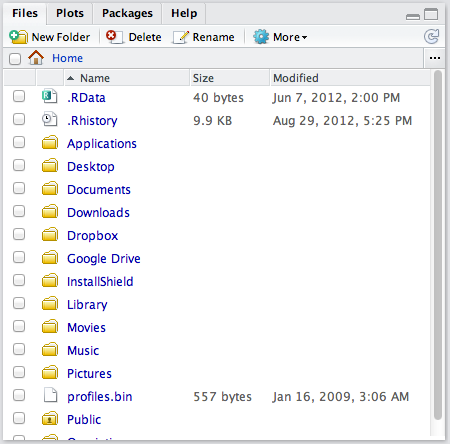
\includegraphics[scale=0.4]{/git_repositories/Rep-Res-Book/Source/Children/Chapter4/images4/RStudioFiles.png}
        \end{center}
\end{figure}



% Part 2, include child documents
\part{Data Gathering and Storage}







